\documentclass[../main.tex]{subfiles}
\graphicspath{{\subfix{../../images/}}}
\begin{document}

\subsection{Learning Metrics}

\begin{figure}[H]
    \makebox[\linewidth][c]{%
        \centering
        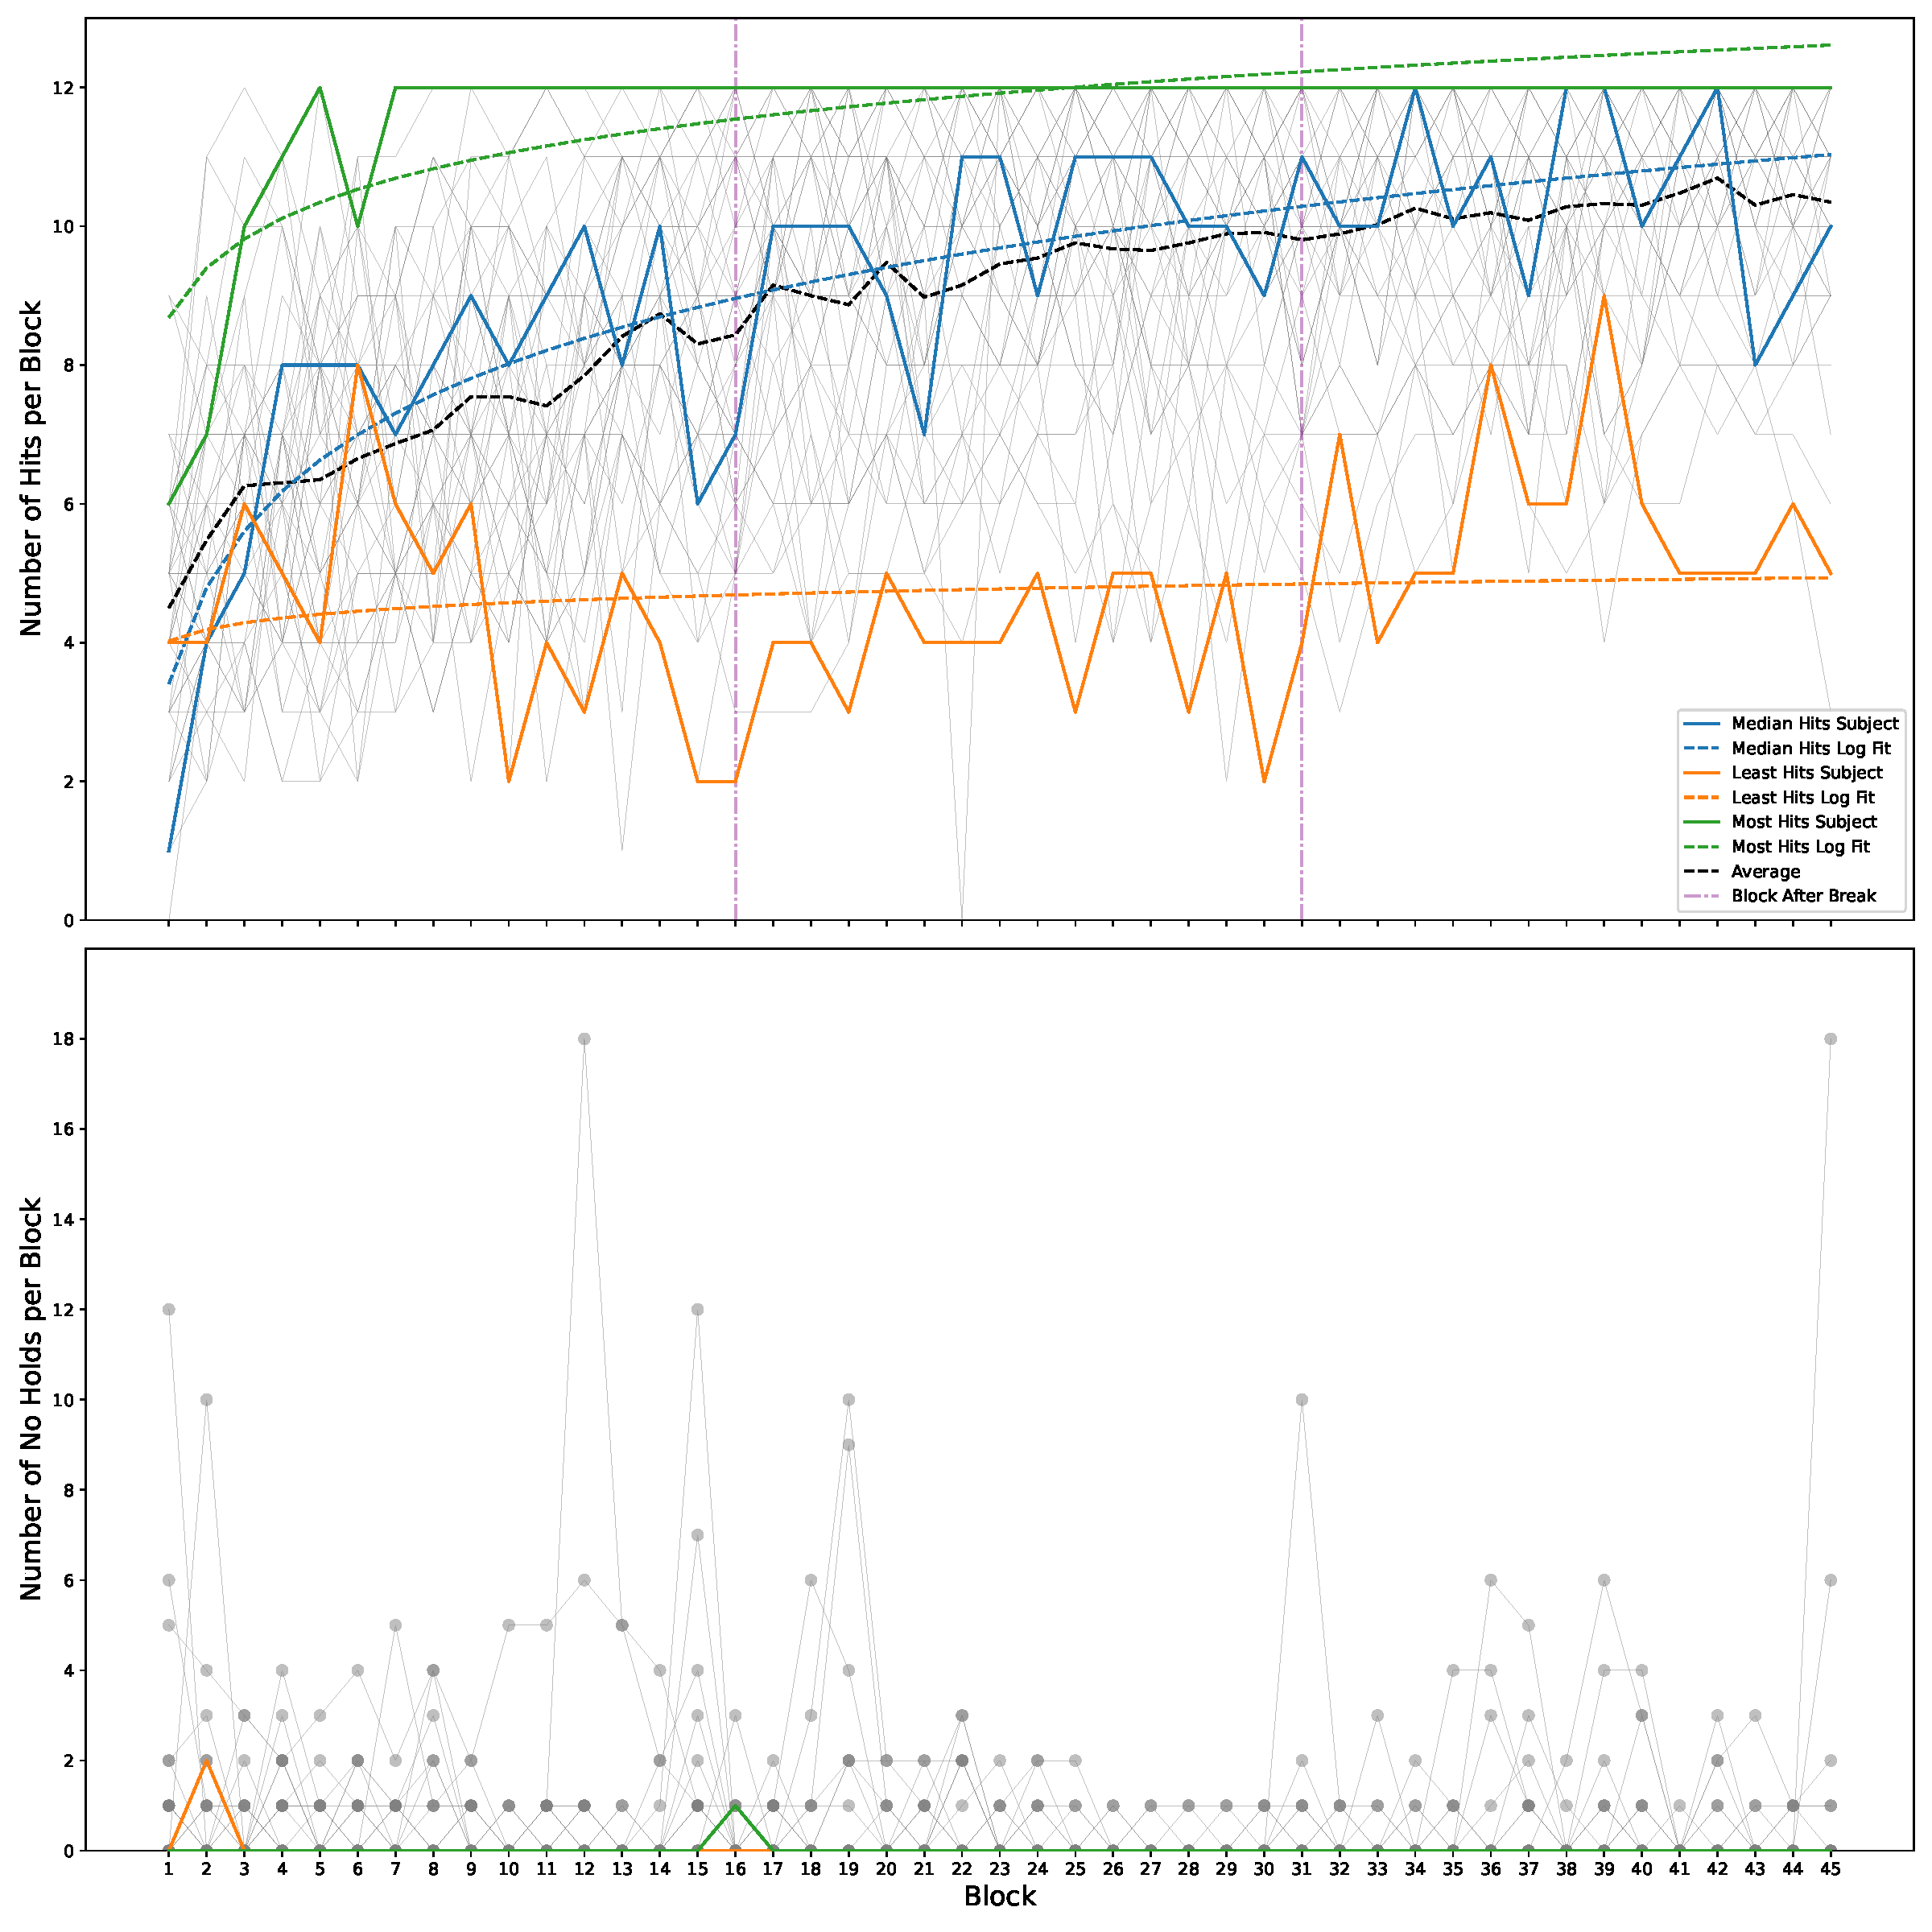
\includegraphics[width=1.3\textwidth]{analysis/hits_and_noholds_over_blocks.pdf}
        }
    \caption{Blah blah blah blah}\label{fig:behavior}
\end{figure}


\begin{figure}[H]
    \makebox[\linewidth][c]{%
        \centering
        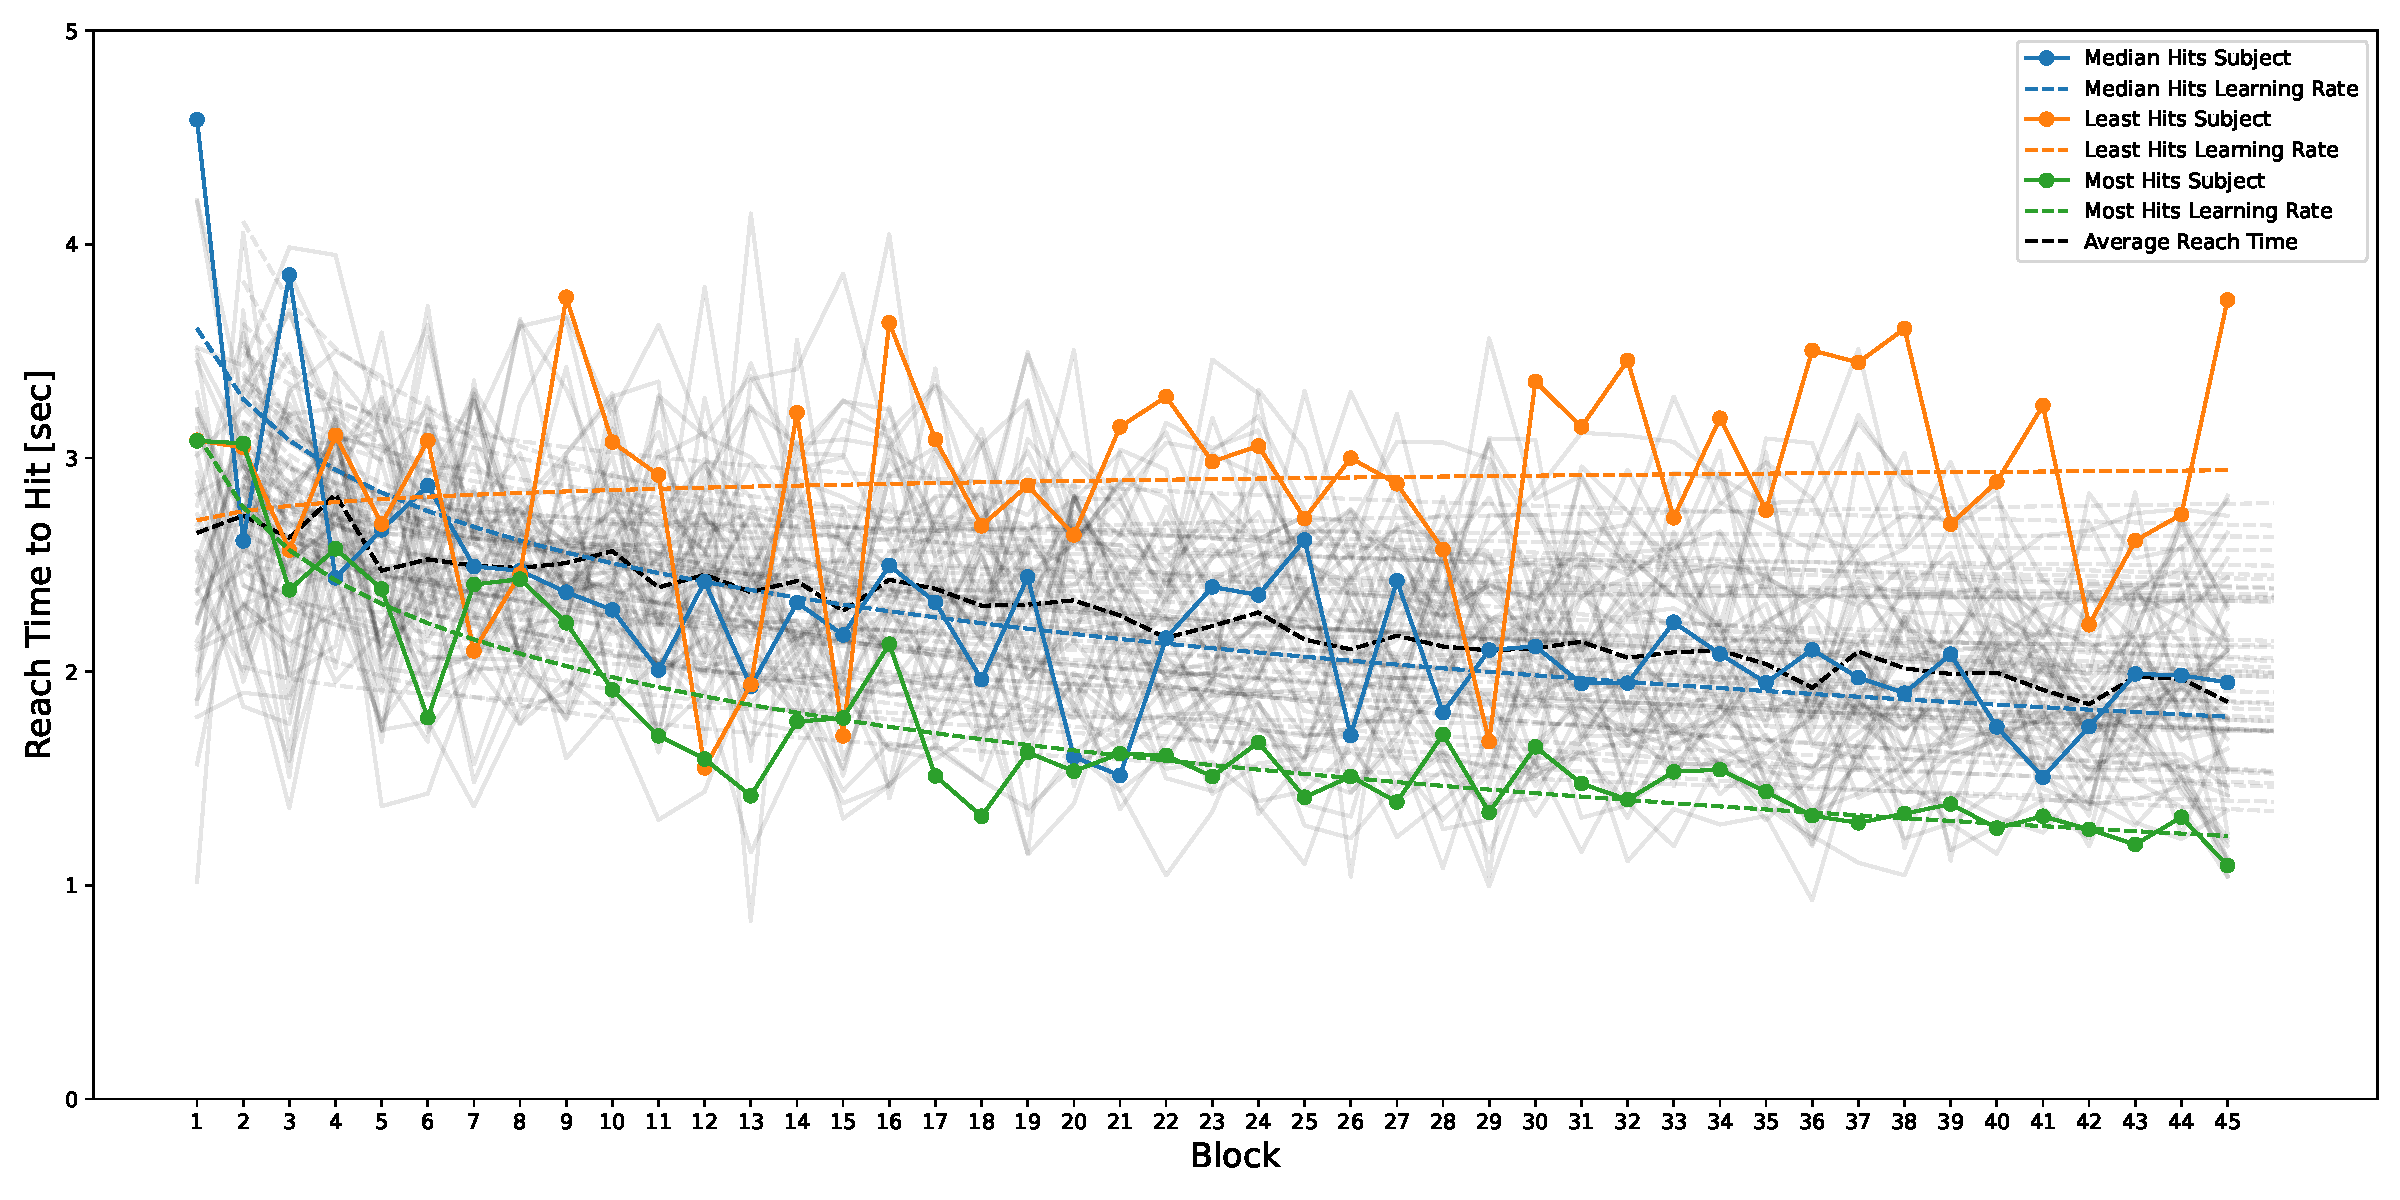
\includegraphics[width=1.3\textwidth]{analysis/reach_times_over_blocks.pdf}
        }
    \caption{Blah blah blah blah}\label{fig:behavior}
\end{figure}


\begin{figure}[H]
    \makebox[\linewidth][c]{%
        \centering
        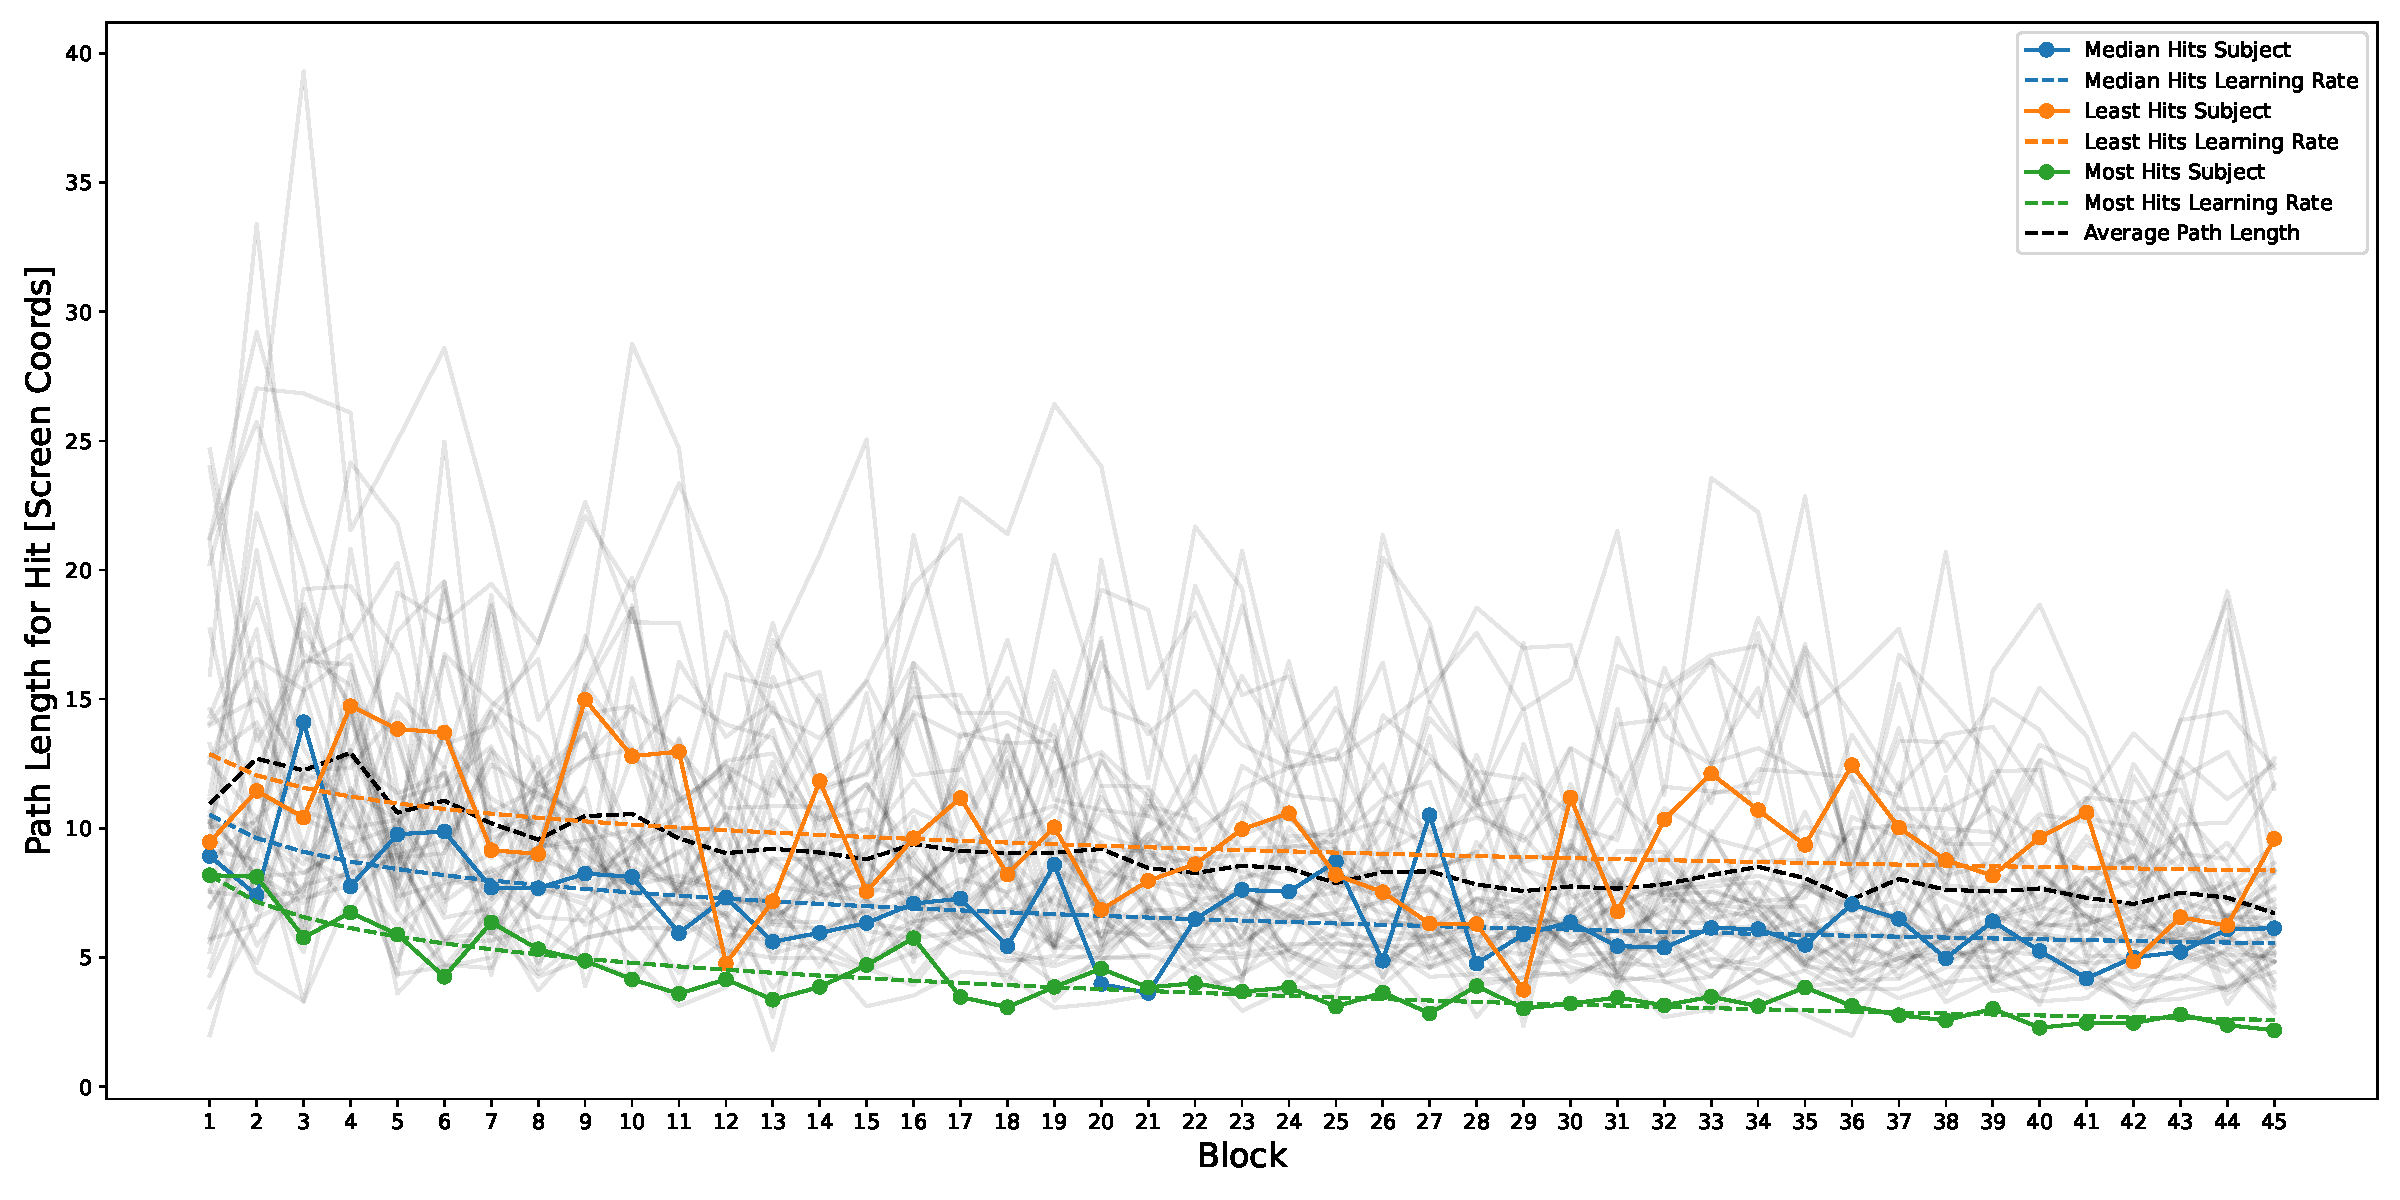
\includegraphics[width=1.3\textwidth]{analysis/path_length_over_blocks.pdf}
        }
    \caption{Blah blah blah blah}\label{fig:behavior}
\end{figure}


\begin{figure}[H]
    \makebox[\linewidth][c]{%
        \centering
        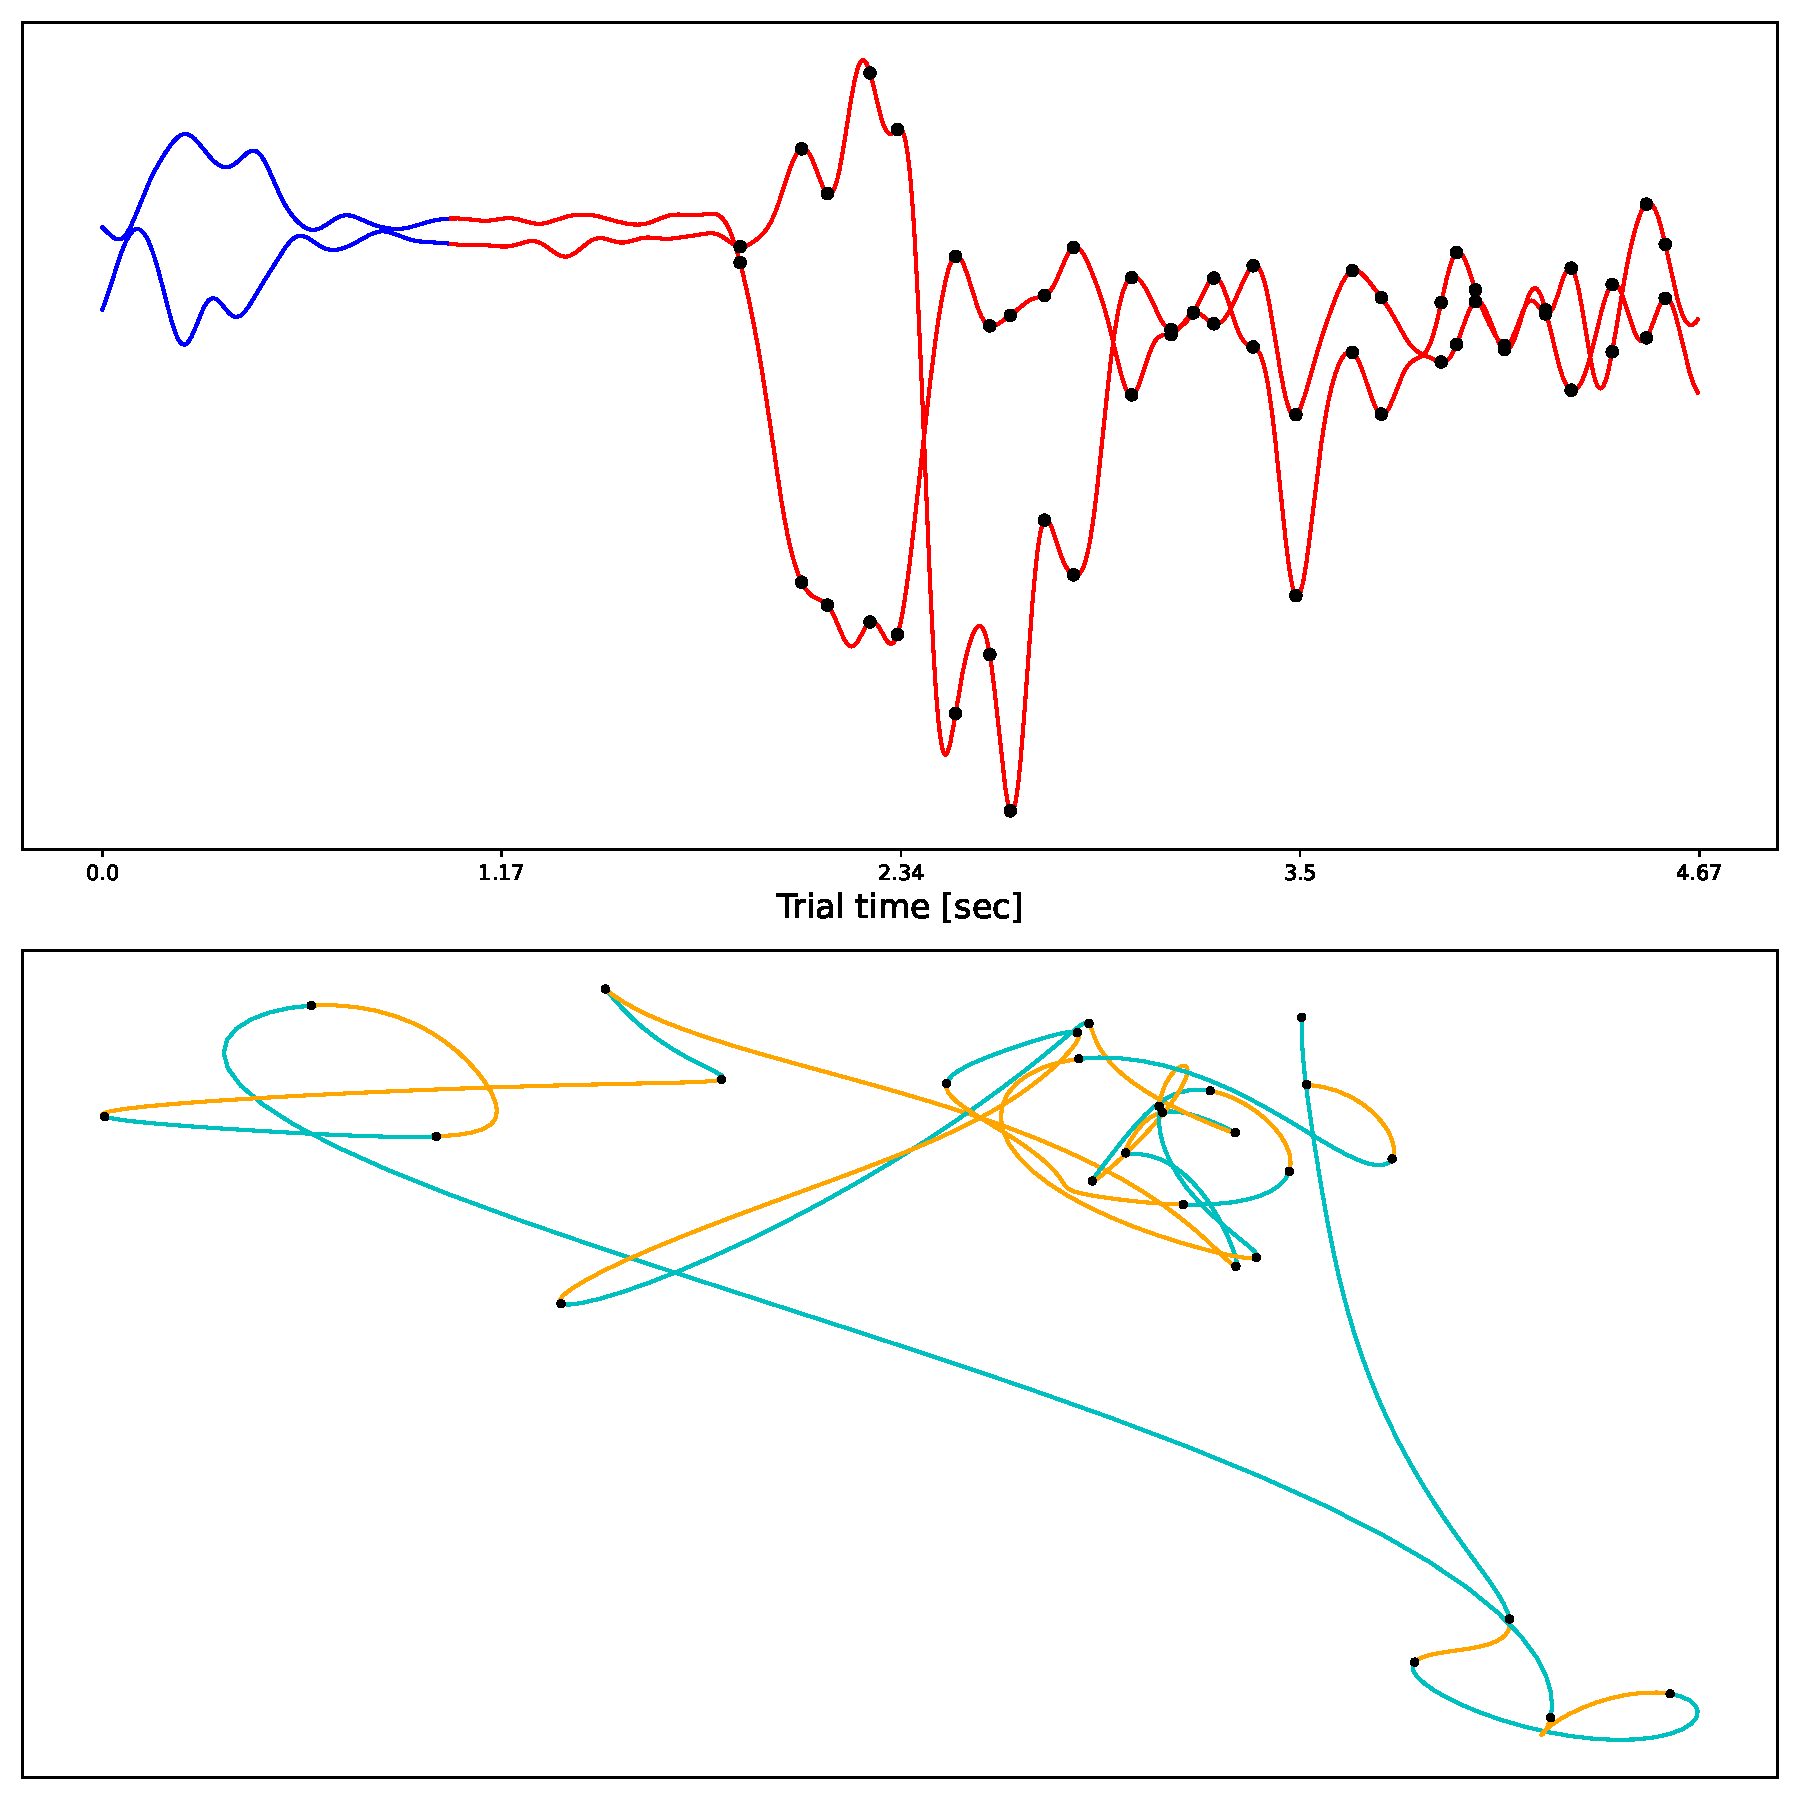
\includegraphics[width=\textwidth]{analysis/example_path_segments.pdf}
    }
    \caption{Blah blah blah blah}\label{fig:behavior}
    \end{figure}


\begin{figure}[H]
    \makebox[\linewidth][c]{%
        \centering
        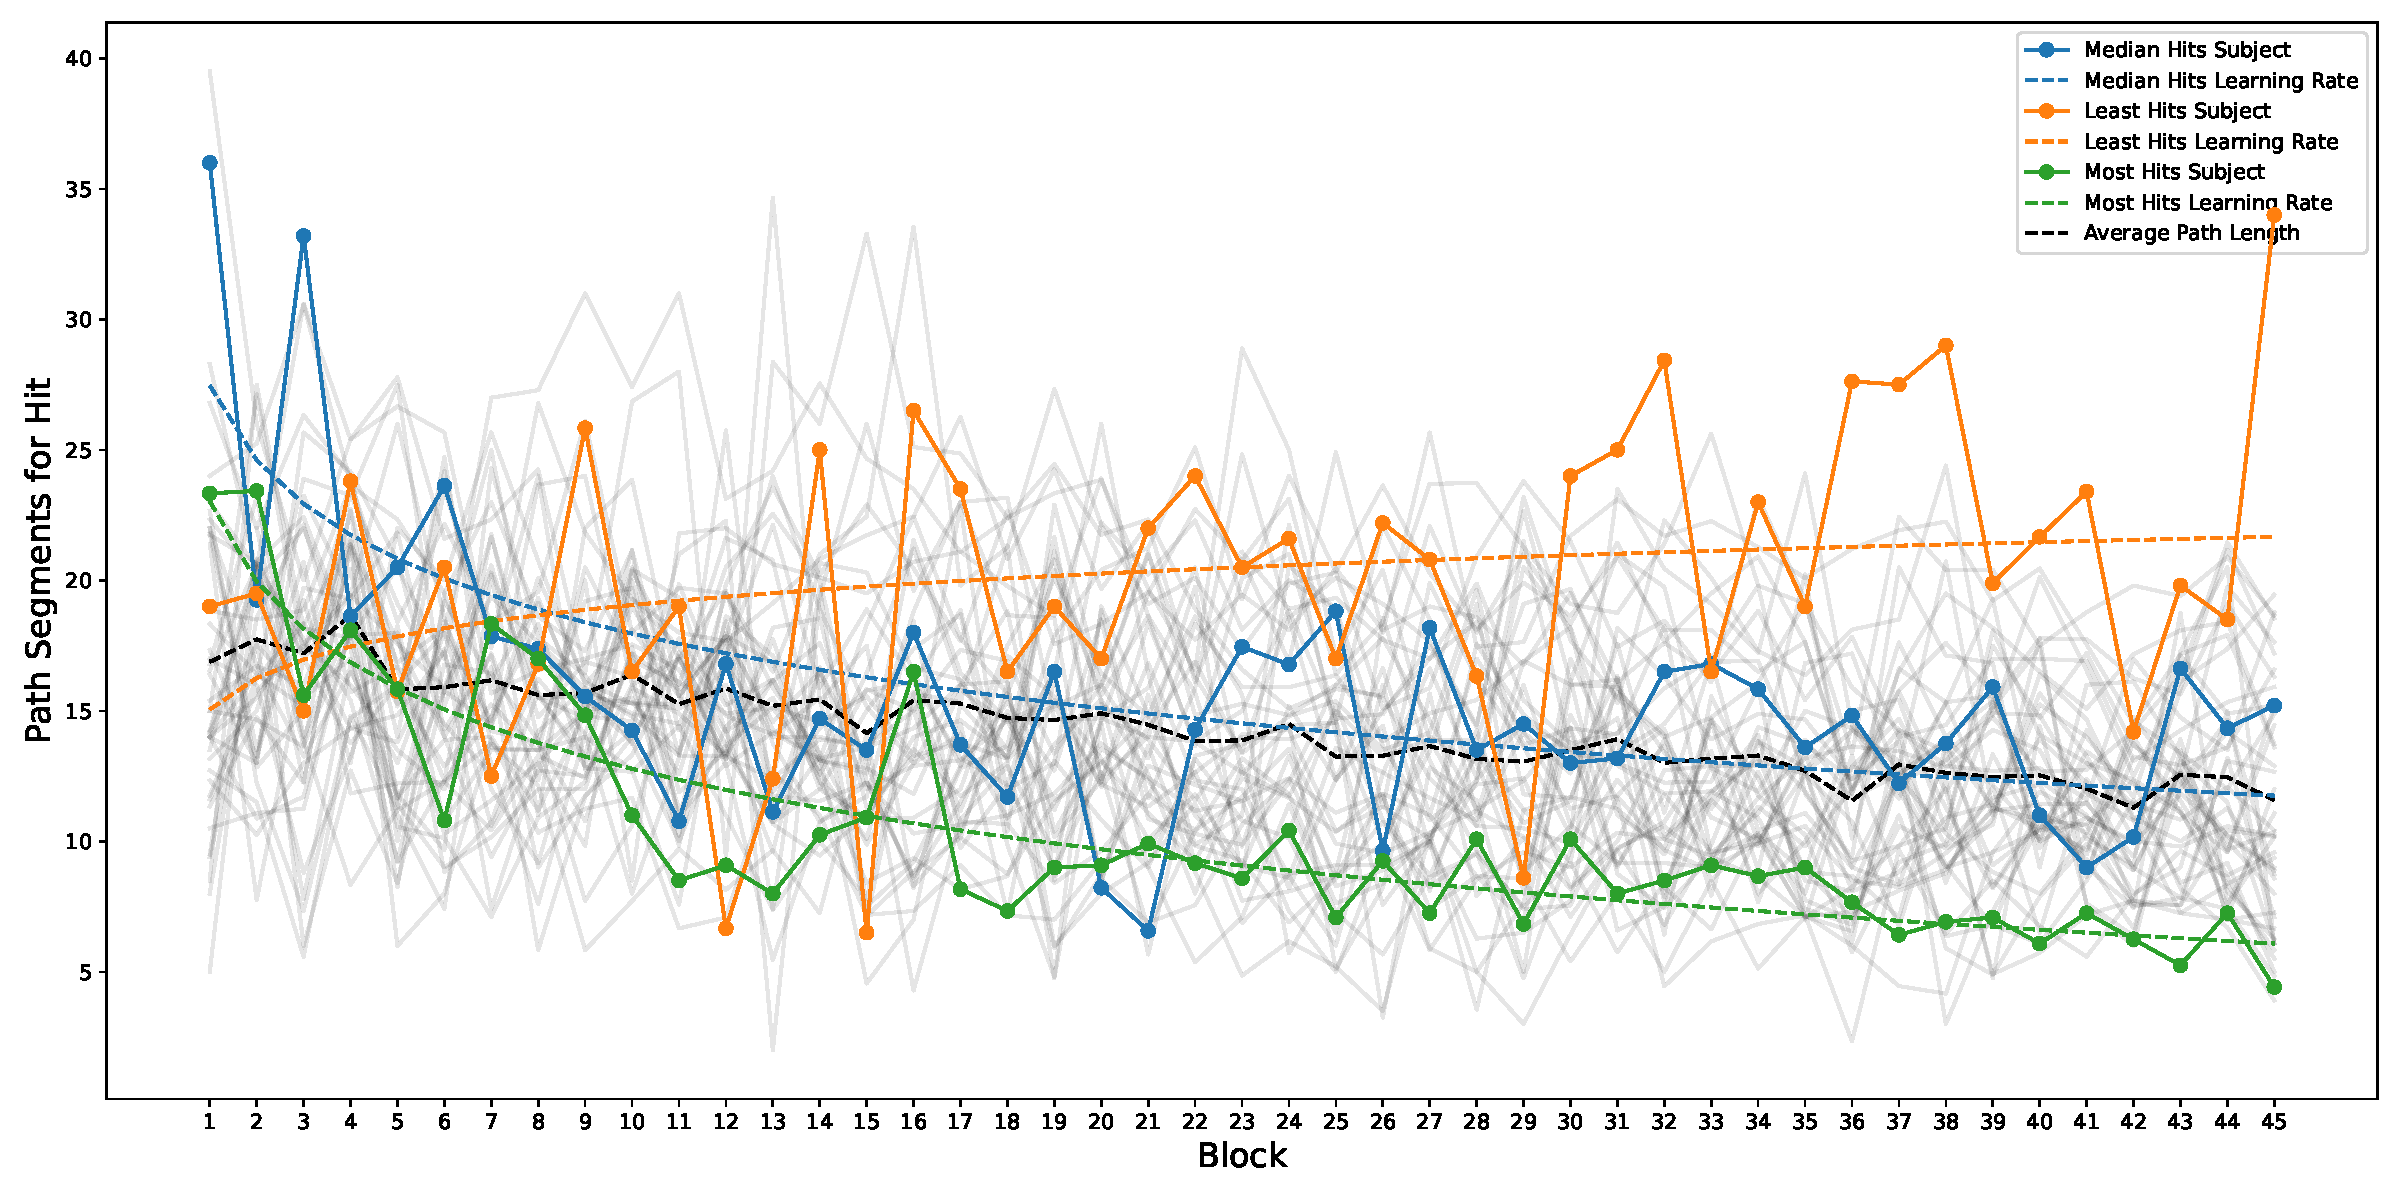
\includegraphics[width=1.3\textwidth]{analysis/segments_over_blocks.pdf}
    }
    \caption{Blah blah blah blah}\label{fig:behavior}
\end{figure}


\begin{figure}[H]
    \makebox[\linewidth][c]{%
        \centering
        \begin{subfigure}{.5\textwidth}
            \centering
            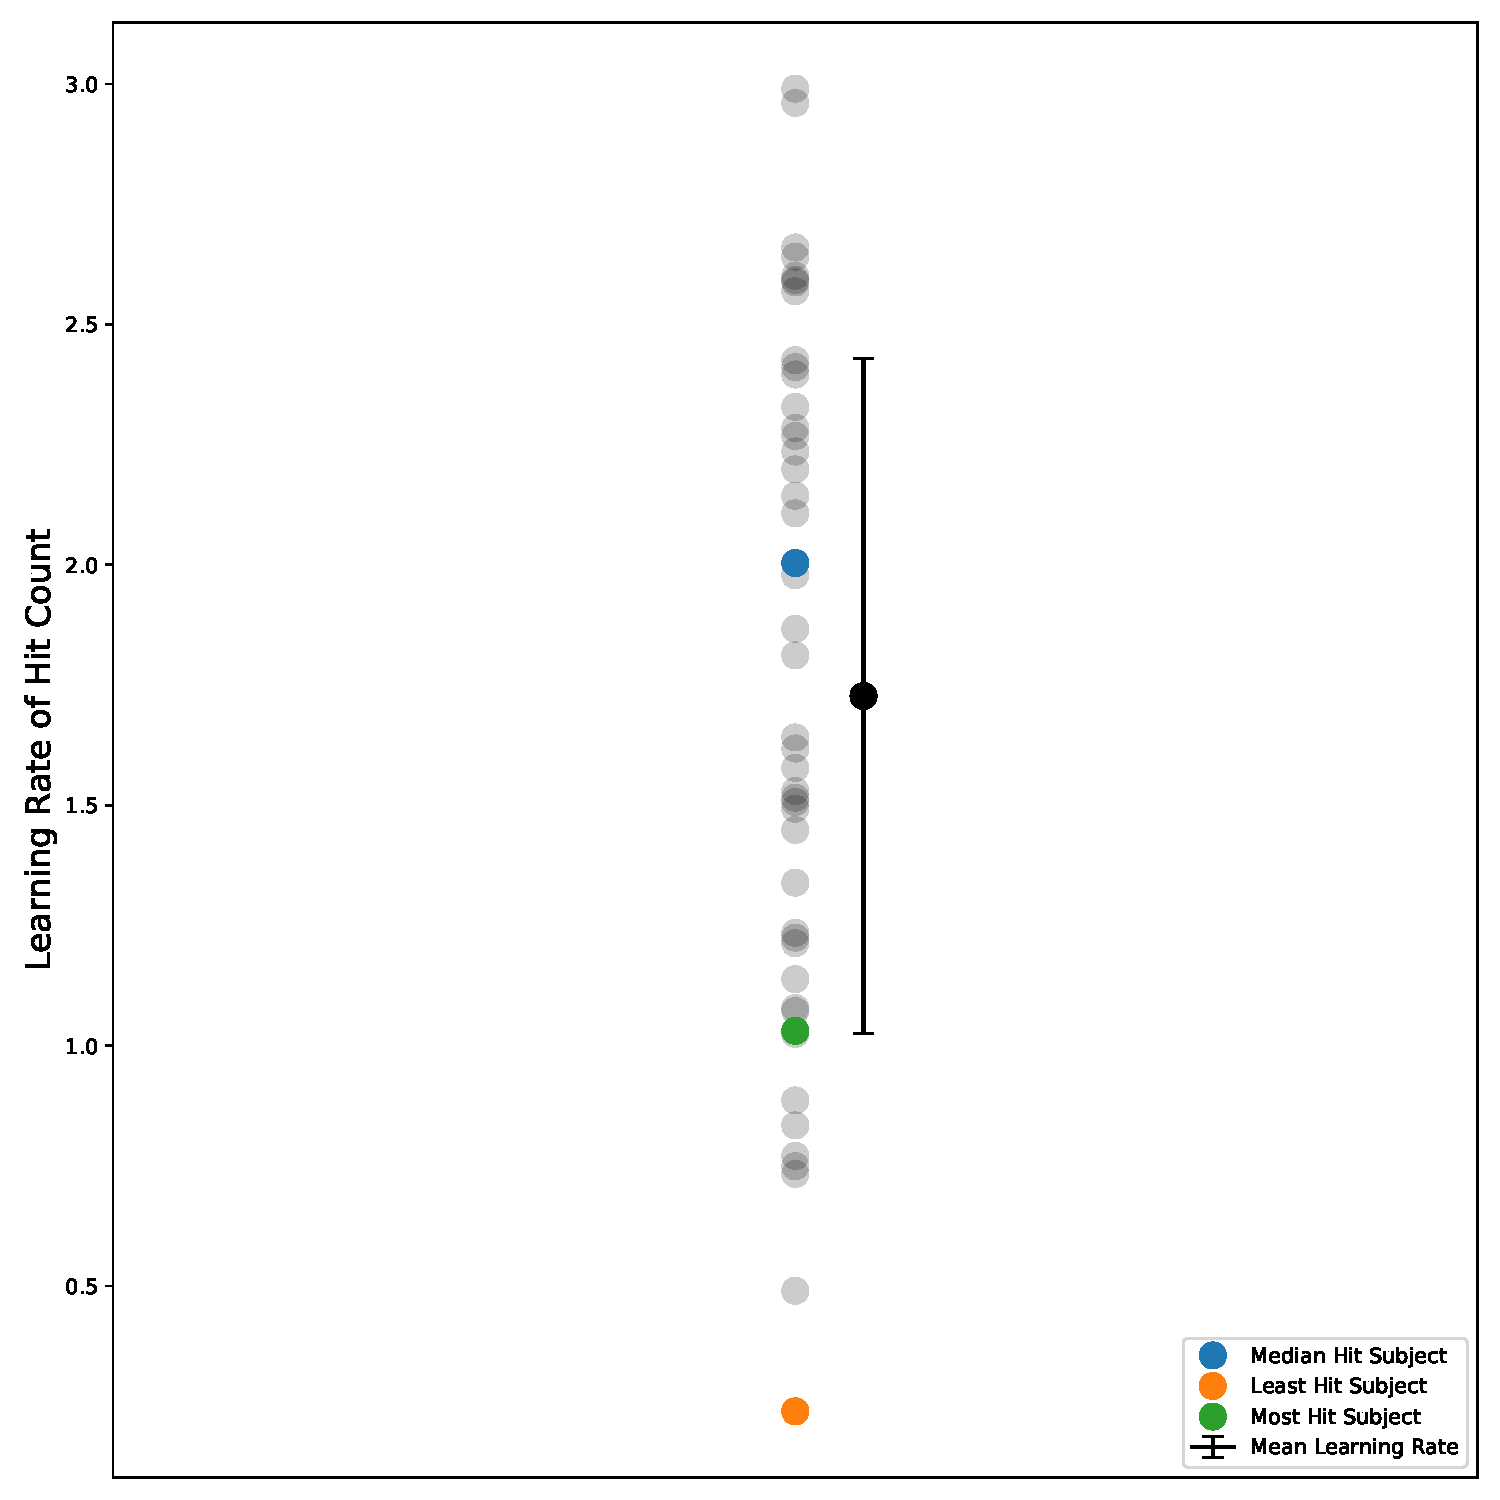
\includegraphics[width=\textwidth]{analysis/hits_learning_rates.pdf}
            \caption{}
            \label{fig:hit_learning_rates}
        \end{subfigure}%
        \begin{subfigure}{.5\textwidth}
            \centering
            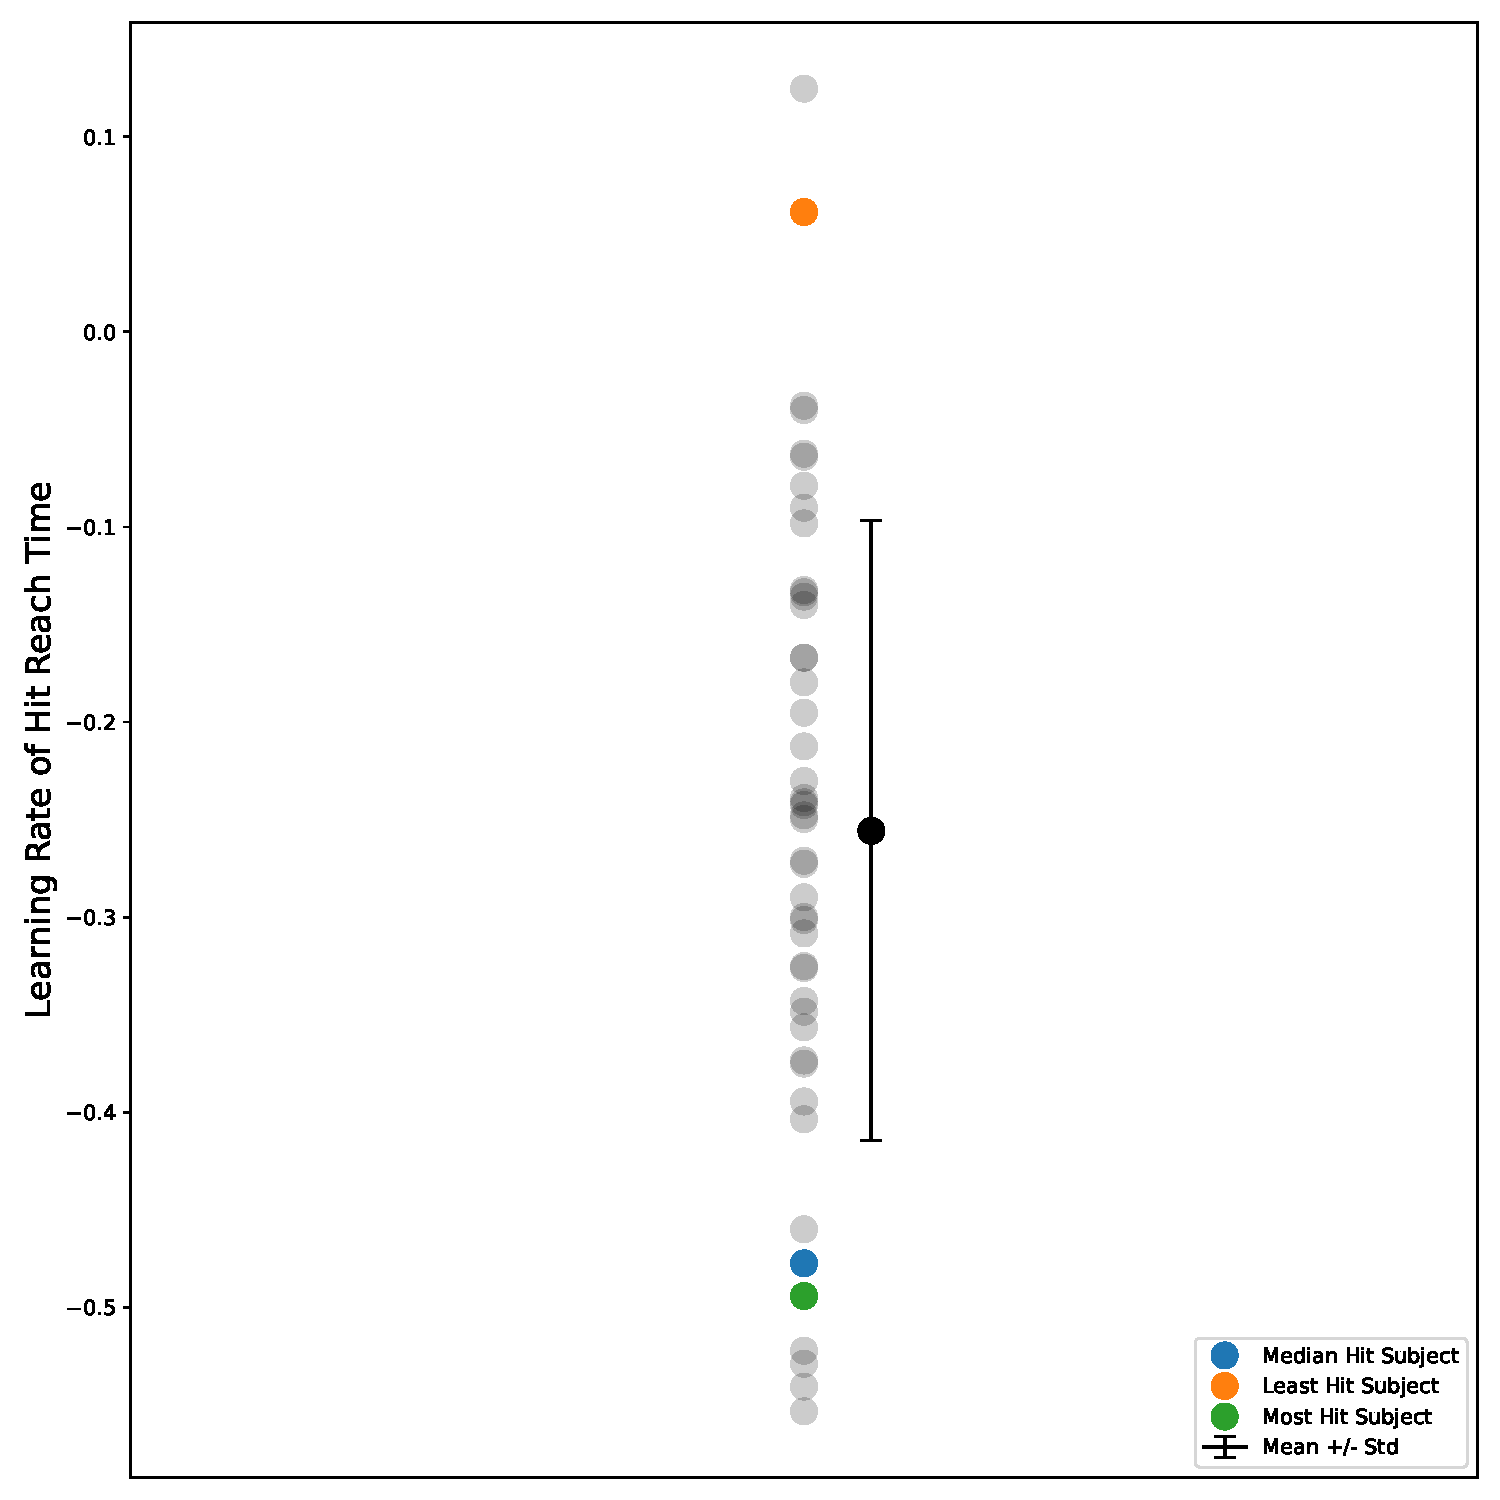
\includegraphics[width=\textwidth]{analysis/reach_time_learning_rates.pdf}
            \caption{}            
            \label{fig:reach_time_learning_rates}
        \end{subfigure}%
    }

    \makebox[\linewidth][c]{%
        \begin{subfigure}{.5\textwidth}
            \centering
            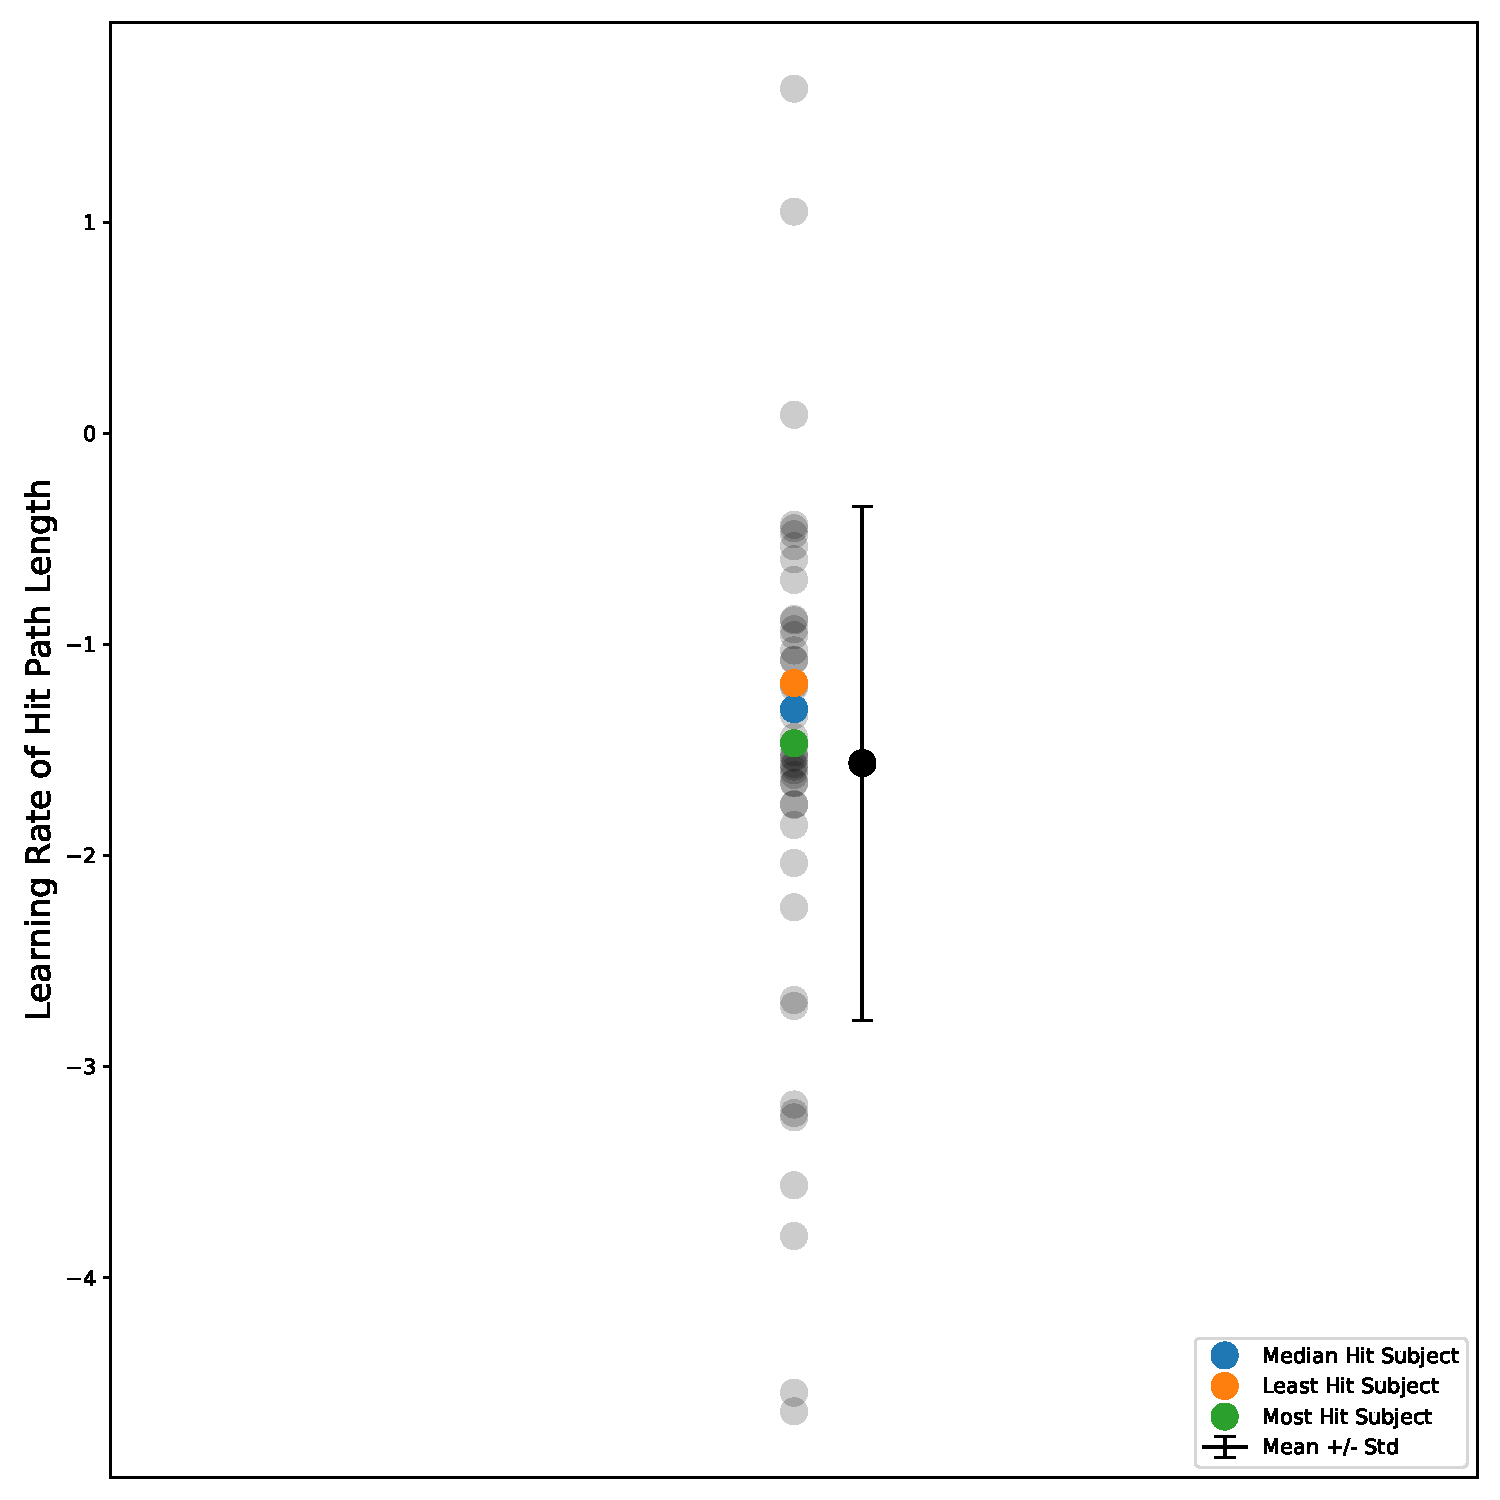
\includegraphics[width=\textwidth]{analysis/path_length_learning_rates.pdf}
            \caption{}            
            \label{fig:path_length_learning_rates}
        \end{subfigure}
        \begin{subfigure}{.5\textwidth}
            \centering
            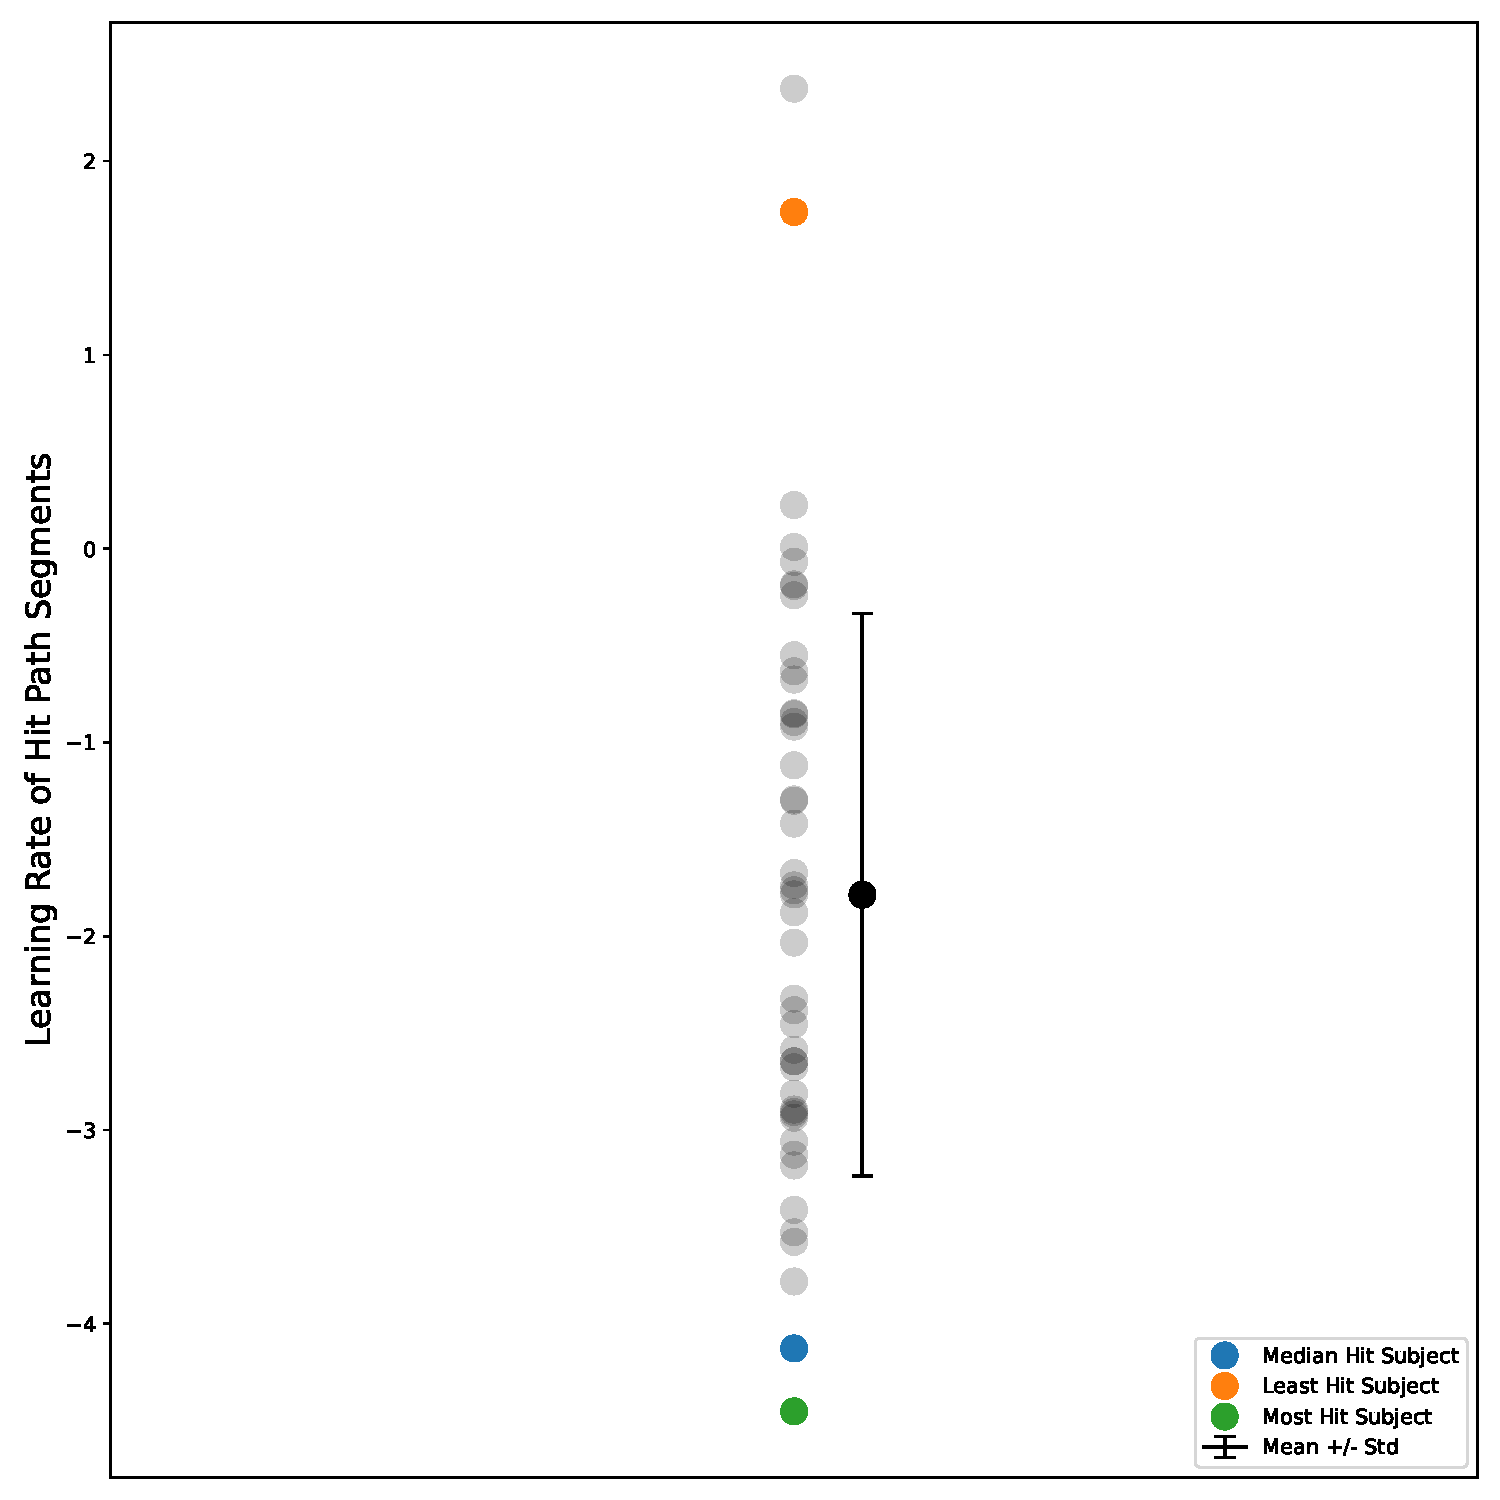
\includegraphics[width=\textwidth]{analysis/segment_learning_rates.pdf}
            \caption{}            
            \label{fig:path_length_learning_rates}
        \end{subfigure}
    }
    \caption{Learning rates for different measures of performance}
    \label{fig:three graphs}
\end{figure}


\begin{figure}[H]
    \makebox[\linewidth][c]{%
        \centering
        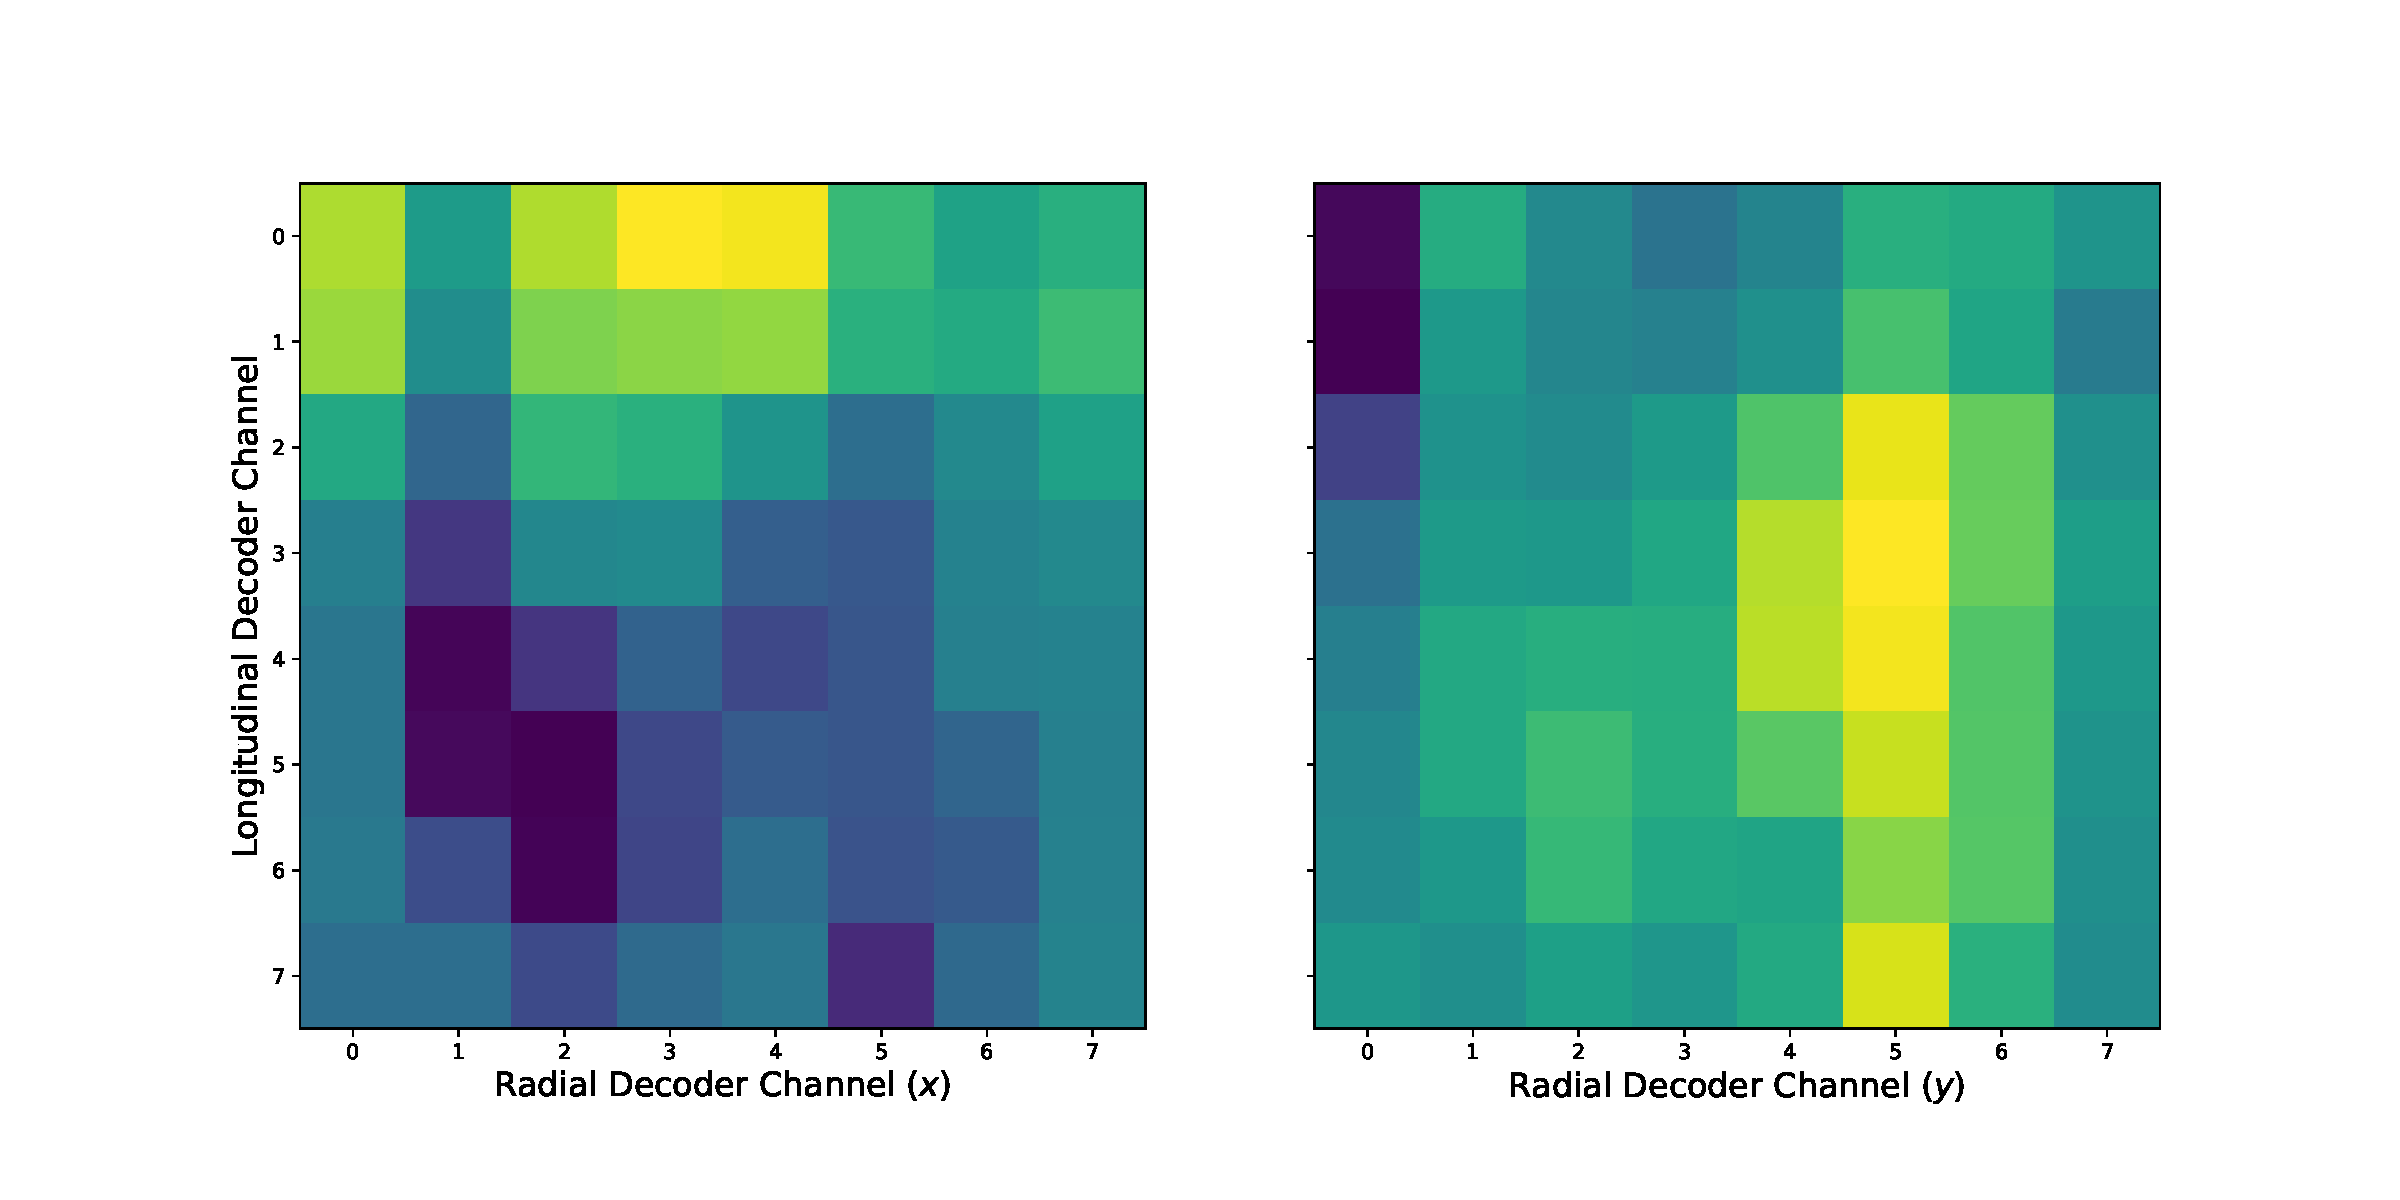
\includegraphics[width=1.4\textwidth]{analysis/example_decoder.pdf}
    }
    \caption{Blah blah blah blah}\label{fig:behavior}
\end{figure}


\begin{figure}[H]
    \makebox[\linewidth][c]{%
        \centering
        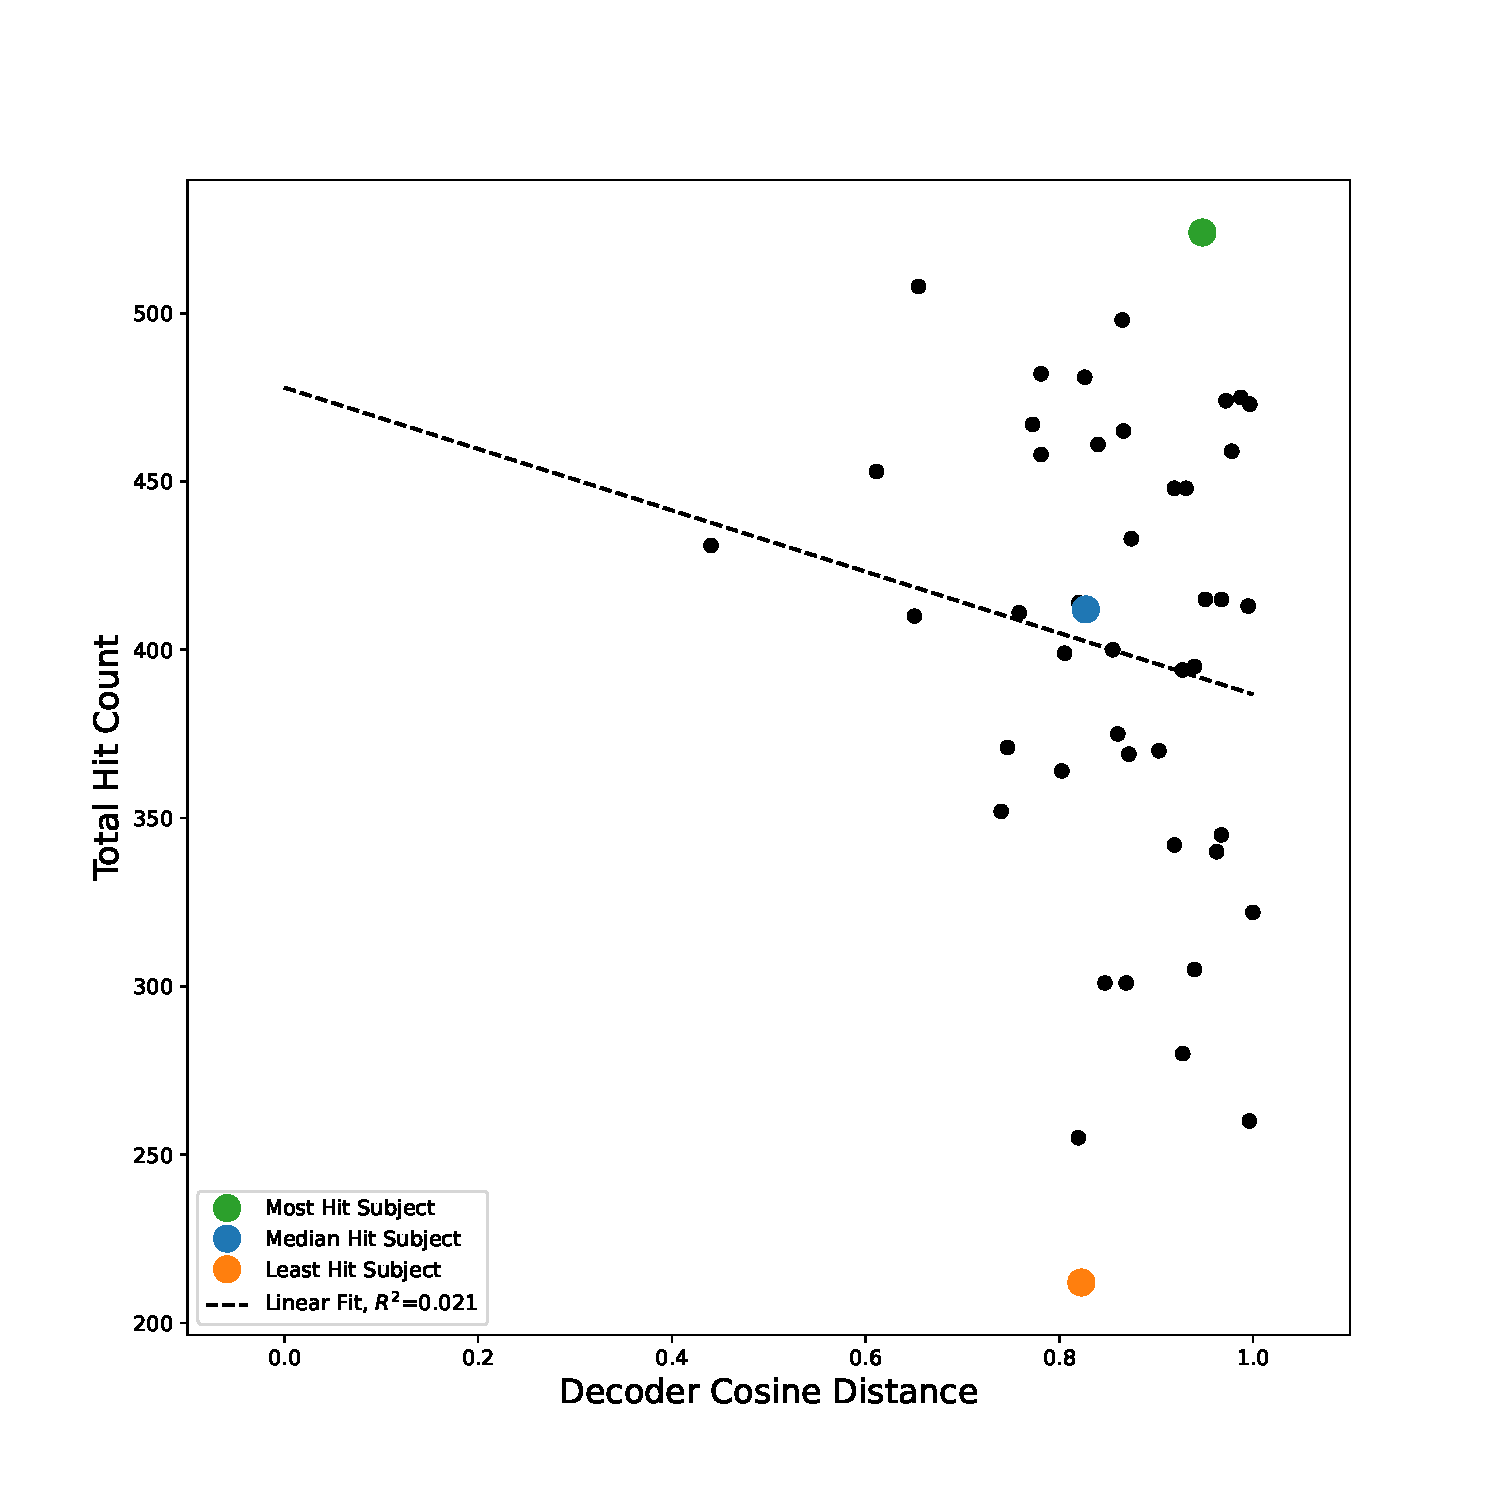
\includegraphics[width=.75\textwidth]{analysis/hit_count_decoder_cosine.pdf}
    }
    \caption{Blah blah blah blah}\label{fig:behavior}
\end{figure}


\begin{figure}[H]
    \makebox[\linewidth][c]{%
        \centering
        \begin{subfigure}{0.7\textwidth}
            \centering
            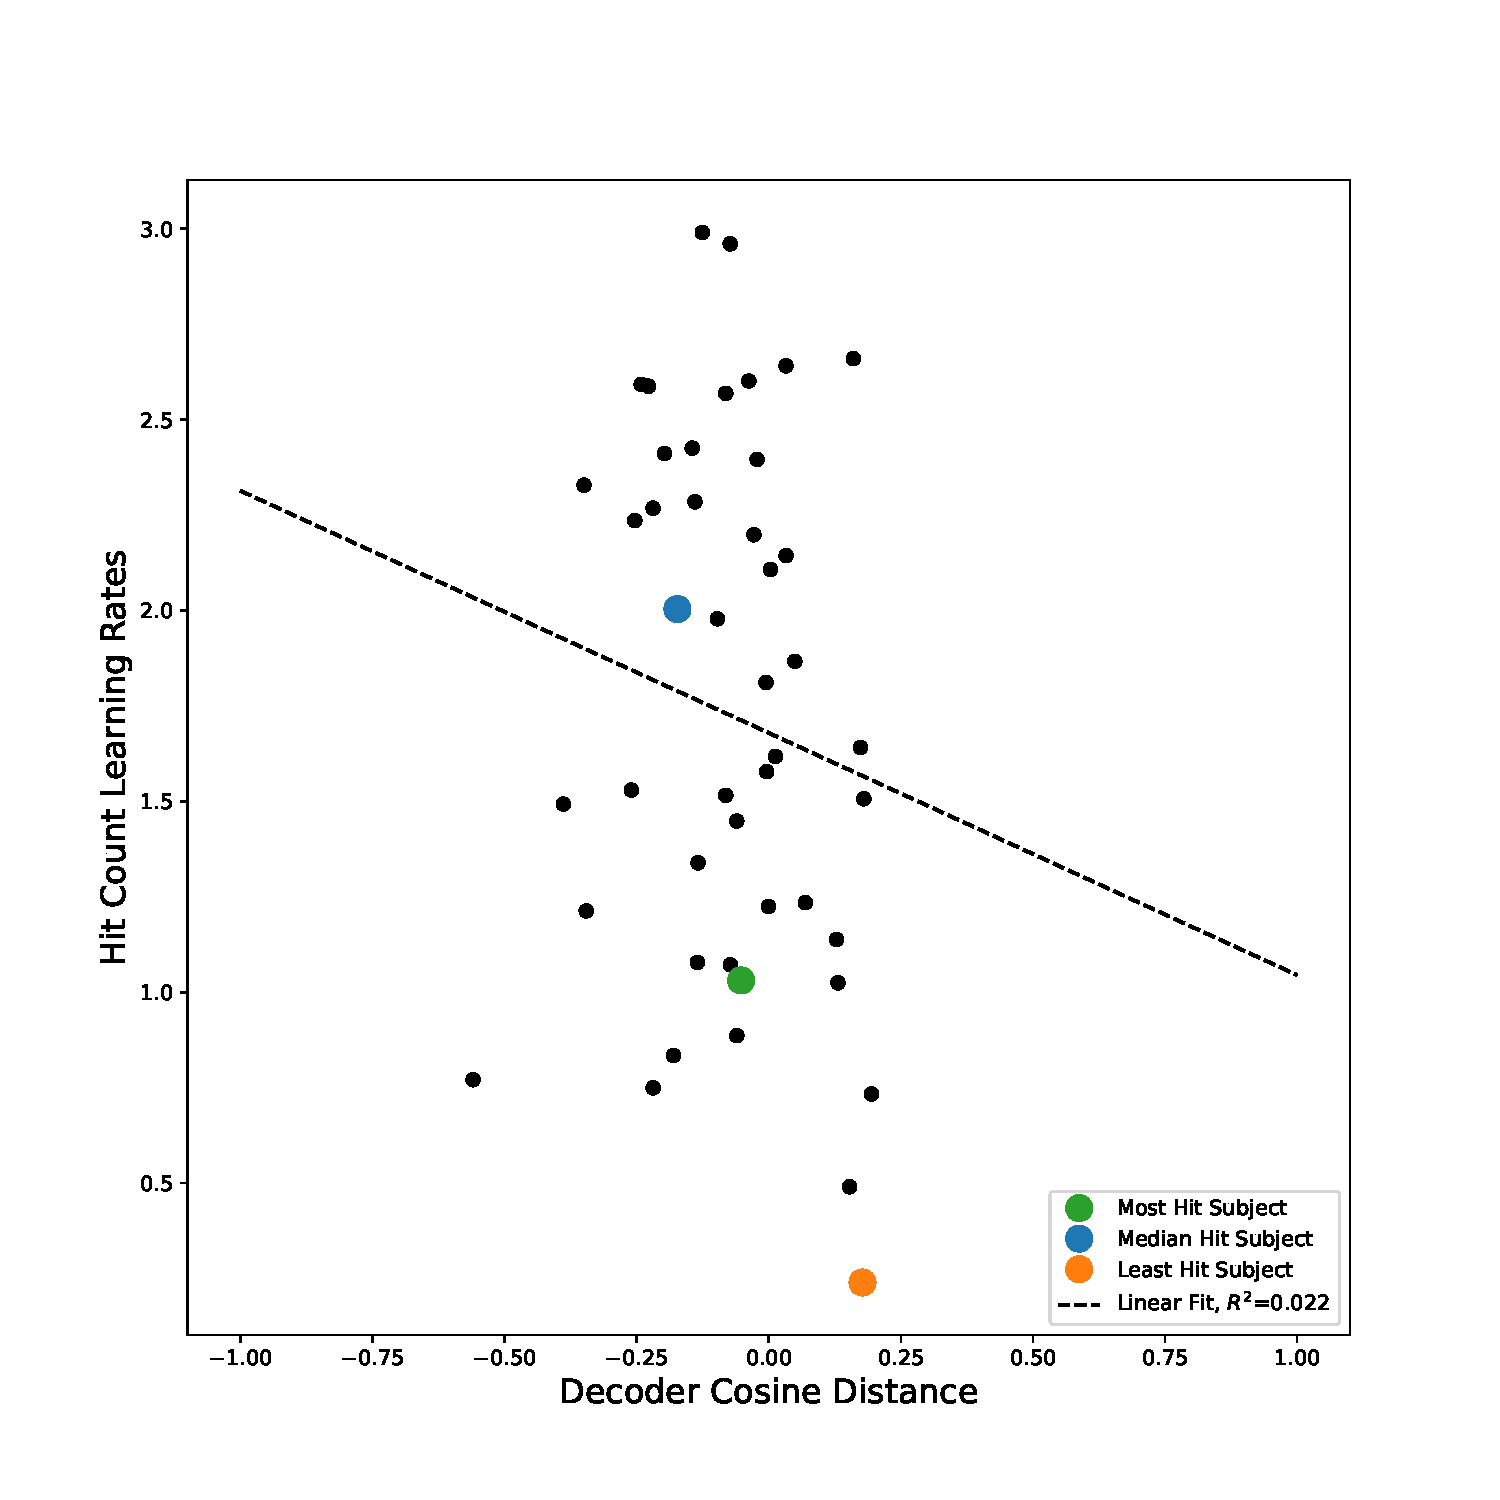
\includegraphics[width=\textwidth]{analysis/hit_lr_decoder_cosine.pdf}
            \caption{}
            \label{fig:hit_learning_rates}
        \end{subfigure}%
        \begin{subfigure}{0.7\textwidth}
            \centering
            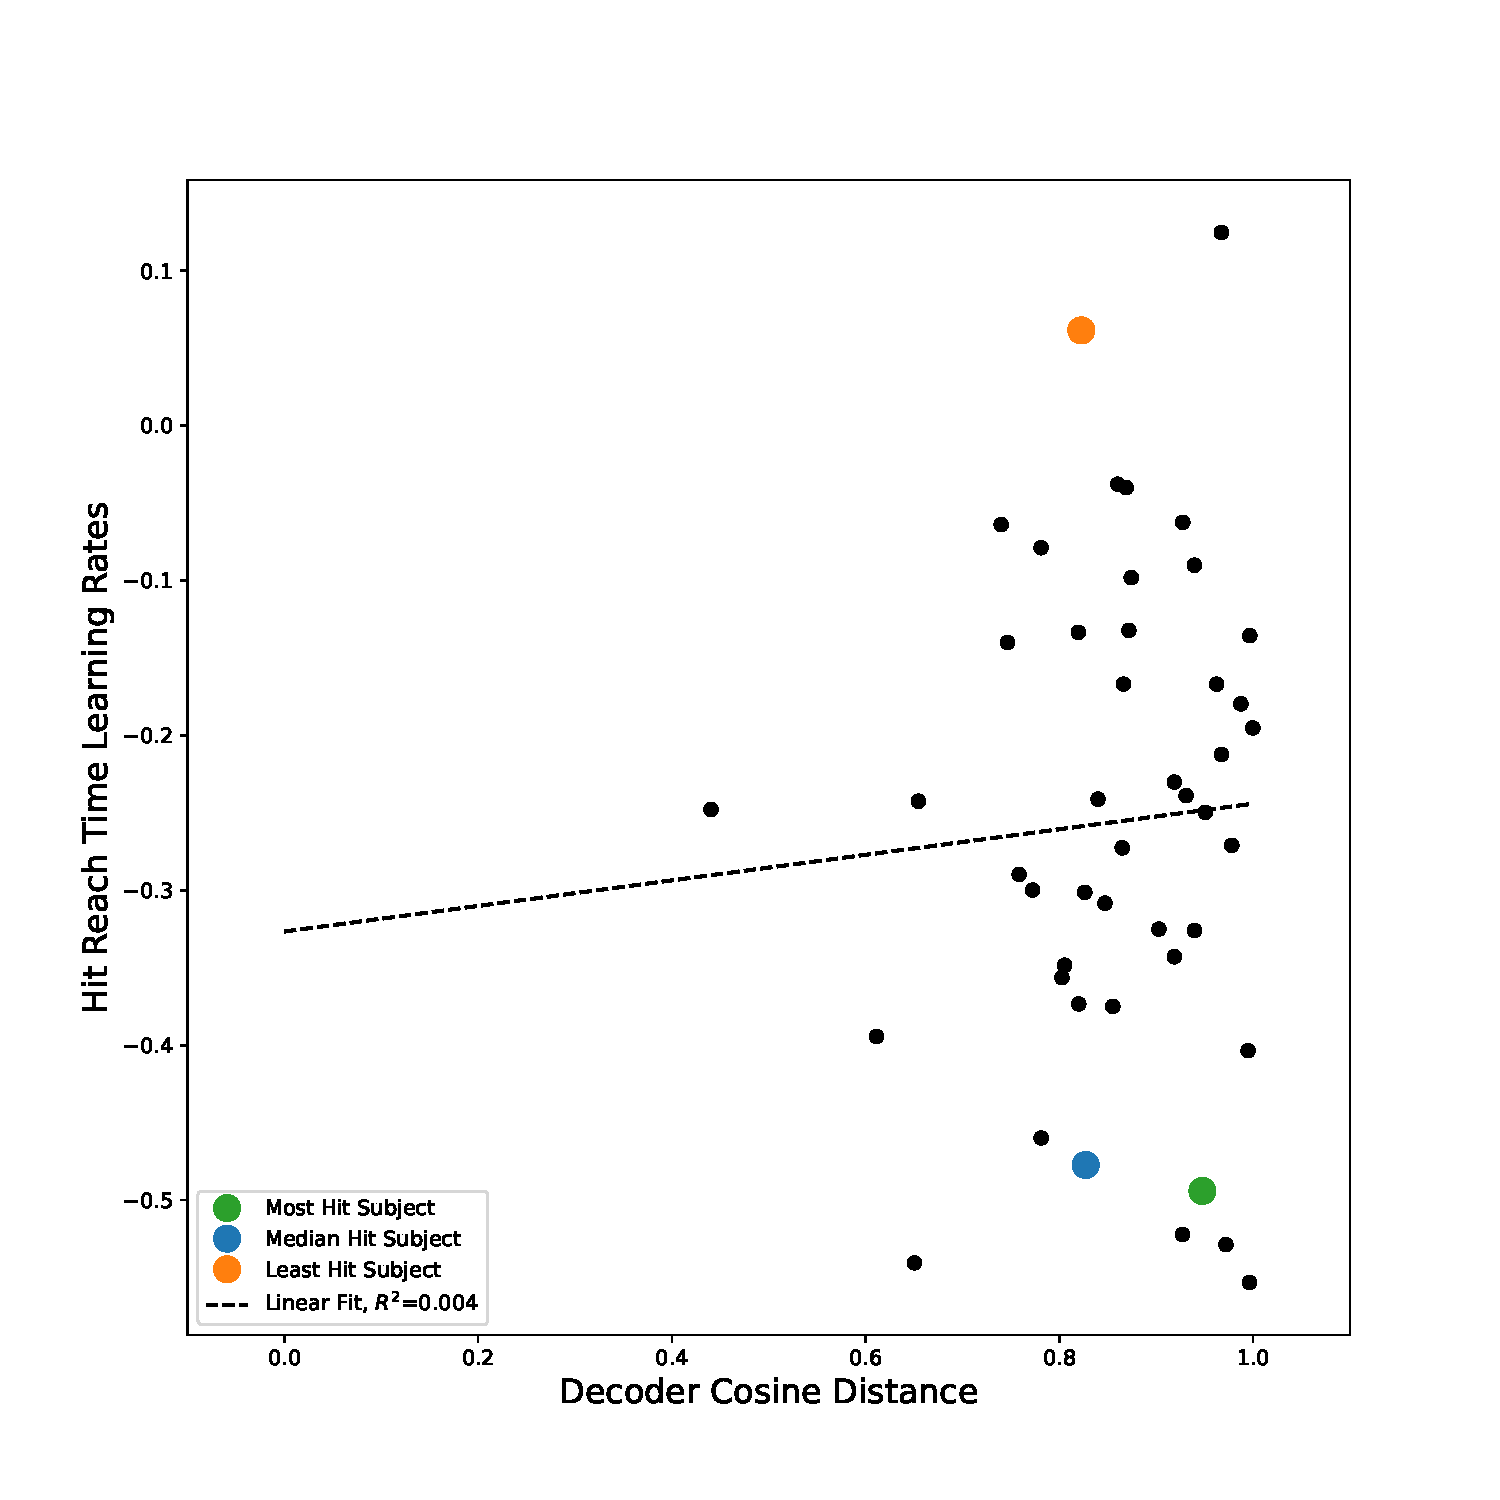
\includegraphics[width=\textwidth]{analysis/reach_time_lr_decoder_cosine.pdf}
            \caption{}            
            \label{fig:reach_time_learning_rates}
        \end{subfigure}
    }

    \makebox[\linewidth][c]{%
        \begin{subfigure}{0.7\textwidth}
            \centering
            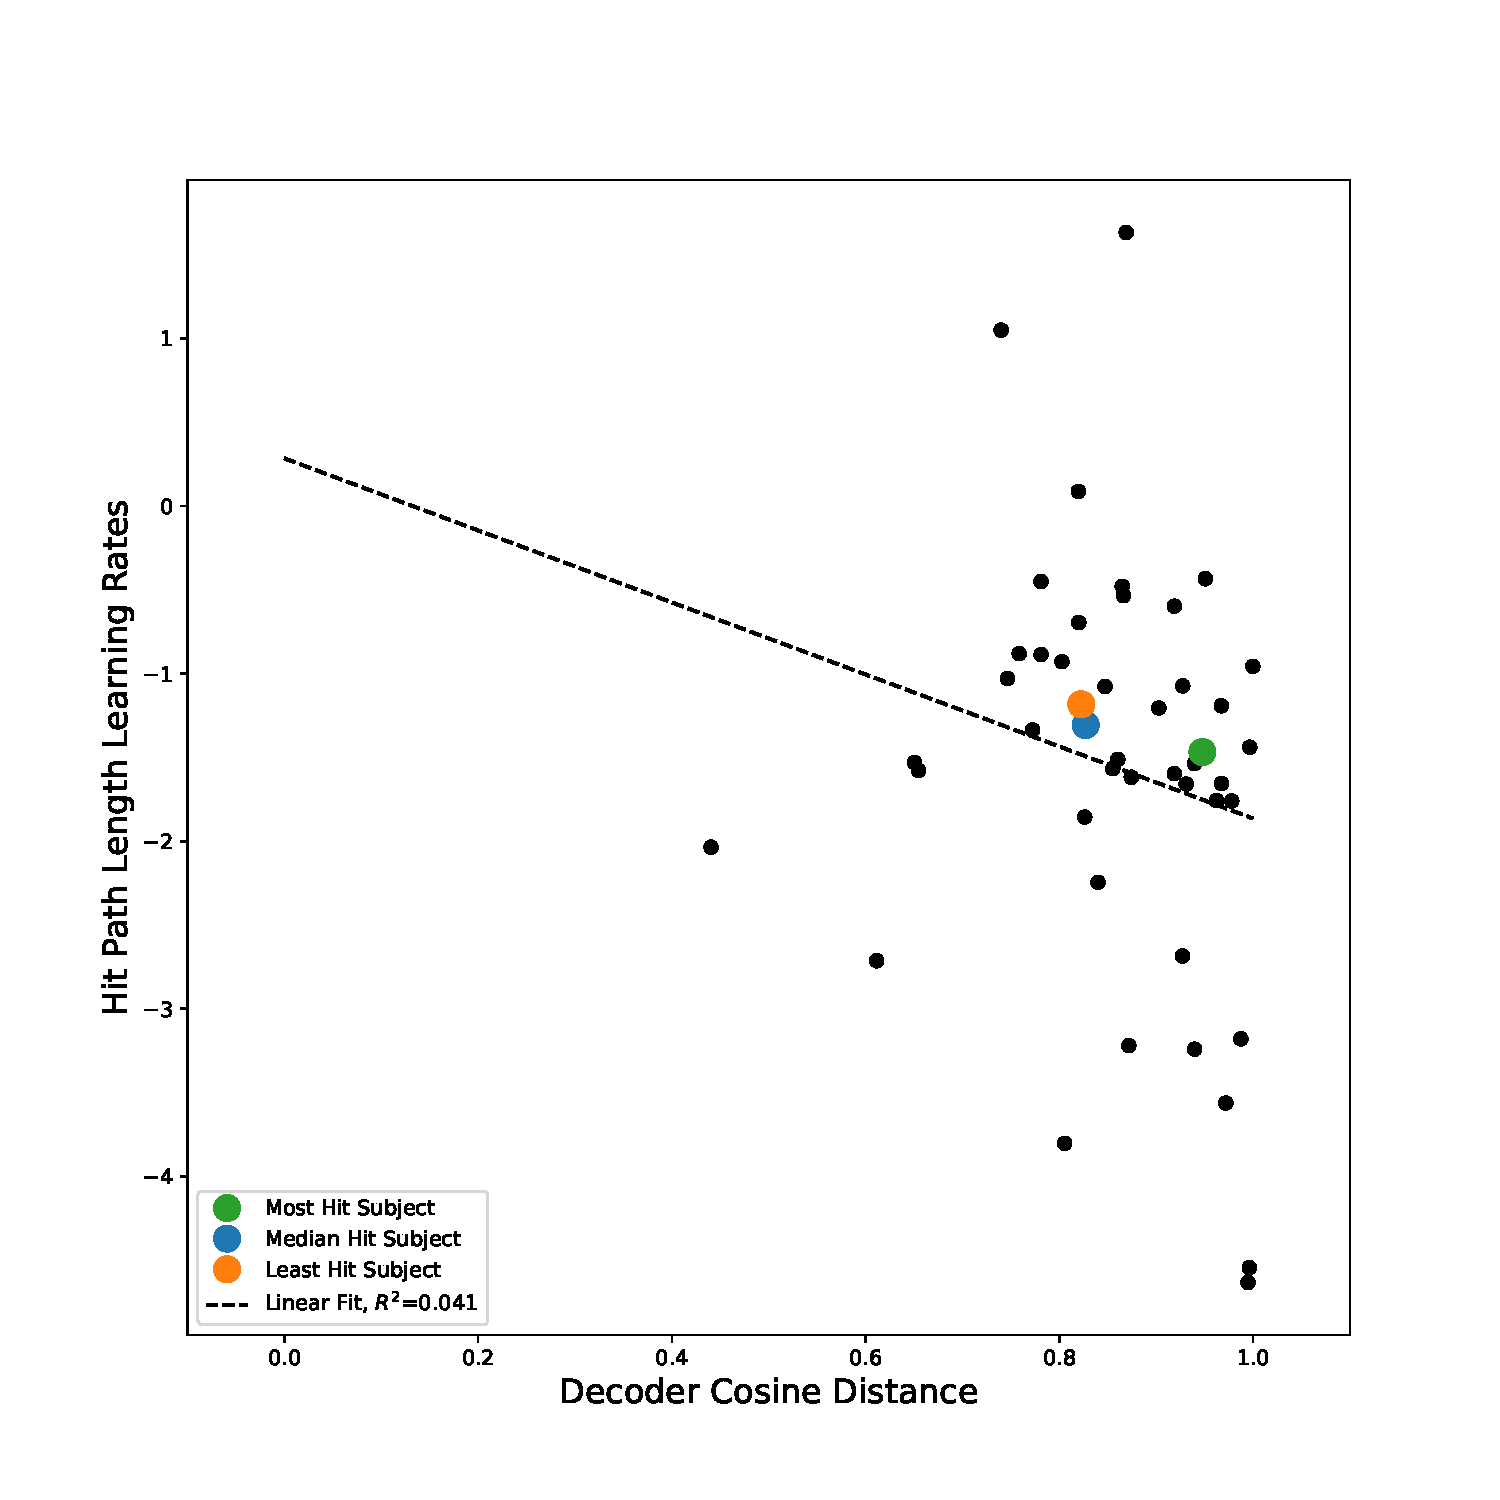
\includegraphics[width=\textwidth]{analysis/path_length_lr_decoder_cosine.pdf}
            \caption{}            
            \label{fig:path_length_learning_rates}
        \end{subfigure}%
        \begin{subfigure}{0.7\textwidth}
            \centering
            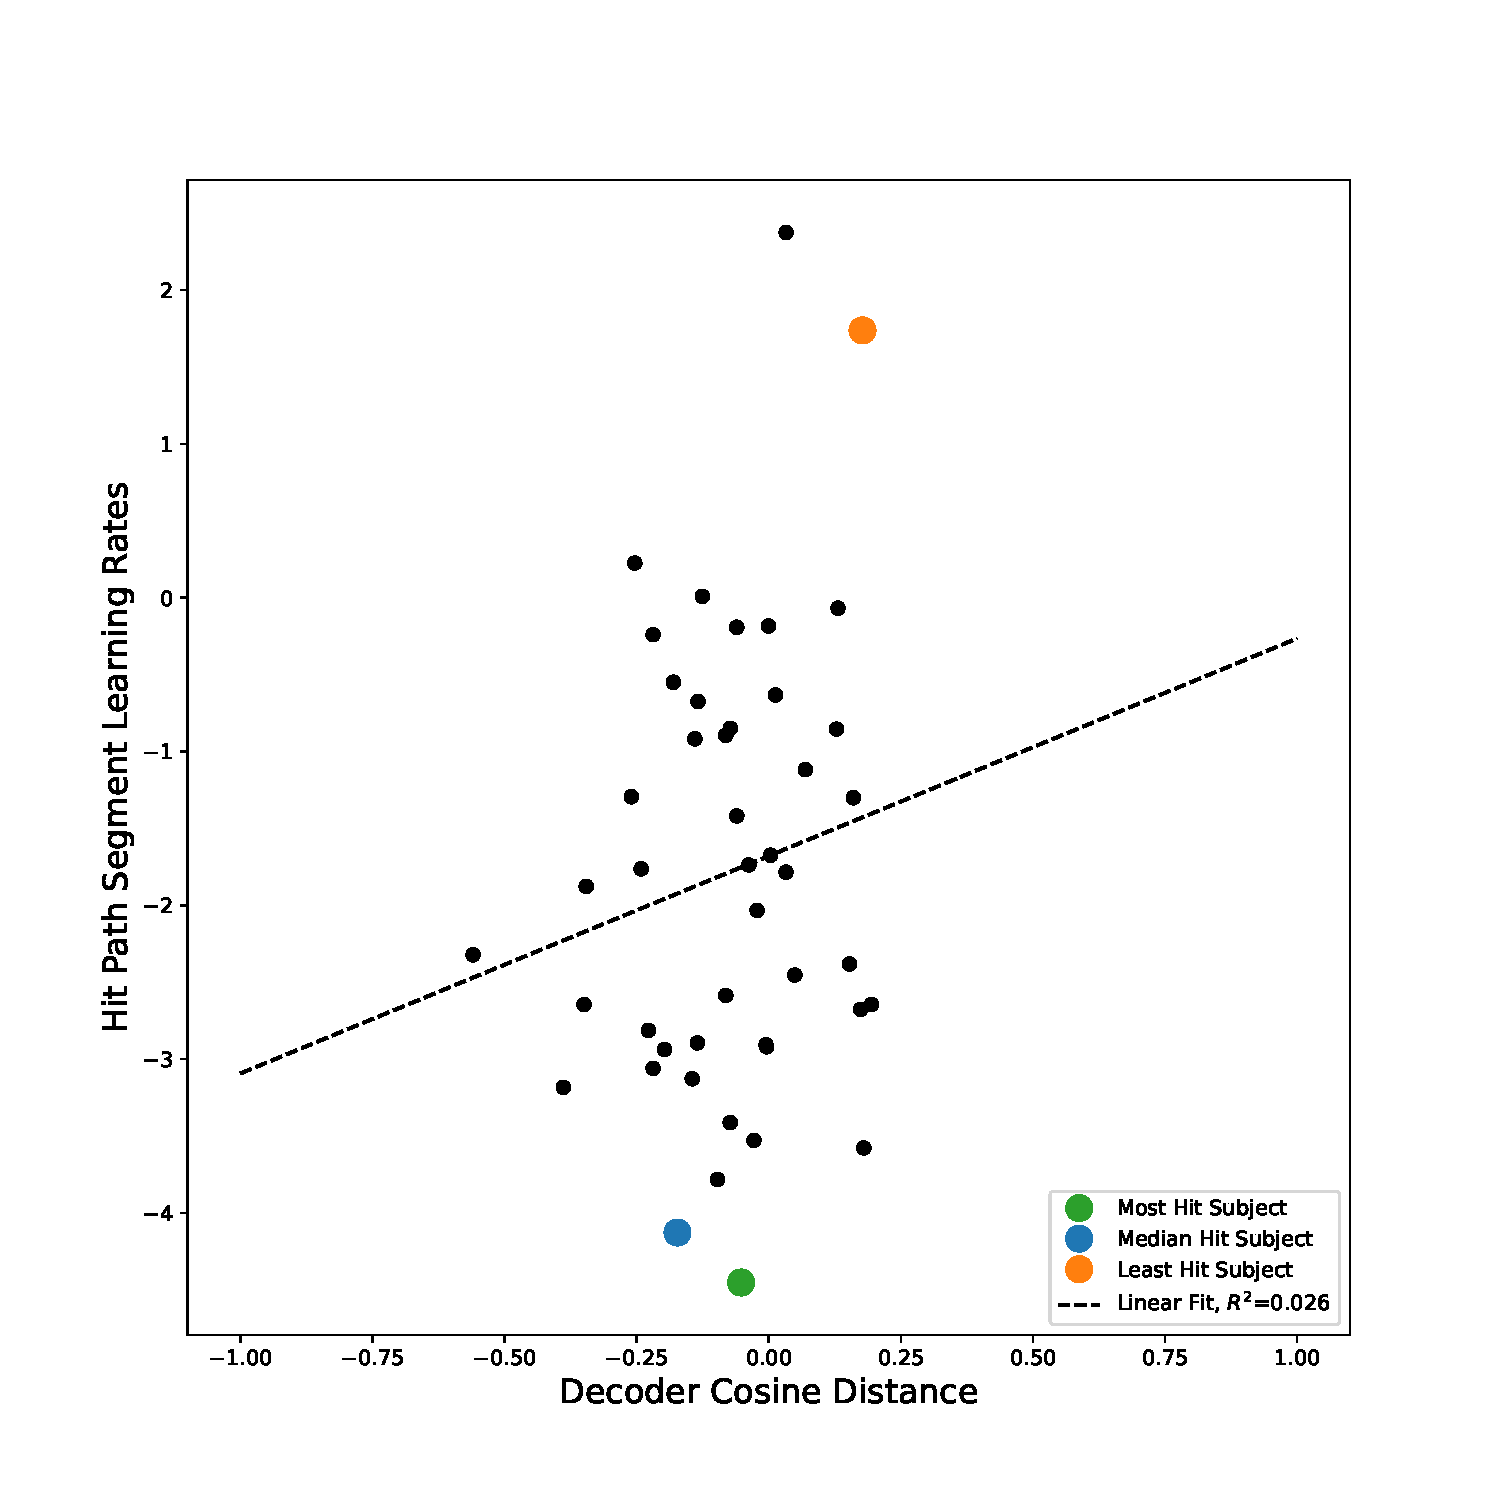
\includegraphics[width=\textwidth]{analysis/segment_lr_decoder_cosine.pdf}
            \caption{}            
            \label{fig:path_length_learning_rates}
        \end{subfigure}%
    }
    \caption{Learning rates for different measures of performance}
    \label{fig:three graphs}
\end{figure}


\end{document}